% research_project_1.tex
% Build with:  latexmk -pdf research_project_1.tex
% or:          pdflatex research_project_1.tex  (run twice so references resolve)

\documentclass[11pt,a4paper]{article}

\usepackage[T1]{fontenc}
\usepackage[utf8]{inputenc}
\usepackage{lmodern}
\usepackage[margin=2.5cm]{geometry}
\usepackage{graphicx}
\usepackage{booktabs}
\usepackage{longtable}
\usepackage{amsmath}
\usepackage{amssymb}
\usepackage{caption}
\usepackage{xcolor}
\usepackage{titlesec}
\usepackage[hidelinks]{hyperref}
\usepackage{enumitem}
\usepackage{setspace}
\usepackage{tocloft}
\usepackage{pdflscape}
\usepackage{float}
\usepackage[section]{placeins}
% Let a page hold more float material before LaTeX defers it to a float page.
% Without this, tables and figures drift several pages away from the text
% that refers to them.
\renewcommand{\topfraction}{0.92}
\renewcommand{\bottomfraction}{0.75}
\renewcommand{\textfraction}{0.06}
\renewcommand{\floatpagefraction}{0.75}
\setcounter{topnumber}{3}
\setcounter{bottomnumber}{2}
\setcounter{totalnumber}{5}
\renewcommand{\cftfigpresnum}{Figure }
\renewcommand{\cfttabpresnum}{Table }
\setlength{\cftfignumwidth}{5.2em}
\setlength{\cfttabnumwidth}{5.2em}

\graphicspath{{../figures/}}
\captionsetup{font=small,labelfont=bf,justification=raggedright,singlelinecheck=false}
\titleformat{\section}{\large\bfseries}{\thesection.}{0.6em}{\MakeUppercase}
\titleformat{\subsection}{\normalsize\bfseries}{\thesubsection}{0.6em}{}
\setlength{\parskip}{0.5em}
\setlength{\parindent}{0pt}
\onehalfspacing
\widowpenalty=10000
\clubpenalty=10000

\newcommand{\gene}[1]{\textit{#1}}

\begin{document}

% ======================================================================
\begin{titlepage}
\centering
\vspace*{0.6cm}

{\large\scshape The University of Manchester\par}
\vspace{0.35cm}
{\normalsize Faculty of Biology, Medicine and Health\par}
\vspace{1.5cm}

\rule{\textwidth}{0.8pt}
\vspace{0.7cm}

{\LARGE\bfseries Towards a Mechanistic Explanation\\[0.35em] of CHD--CKD\par}

\vspace{0.7cm}
\rule{\textwidth}{0.8pt}

\vspace{0.8cm}
{\large Do congenital heart disease and chronic kidney disease\\
share a genetic basis?\par}

\vspace{1.8cm}
{\large\bfseries Research Project 1\par}
\vspace{0.4cm}
{\normalsize BIOL61230\par}

\vspace{1.6cm}
\begin{tabular}{r@{\hspace{1.2em}}l}
\textit{Author:} & Jagadrupa Sahoo \\[0.45em]
\textit{Supervisor:} & Dr David Talavera \\[0.45em]
\textit{Programme:} & MSc Bioinformatics \\
\end{tabular}

\vspace{1.8cm}
{\normalsize 05 February 2022\par}

\vfill
\end{titlepage}

% ======================================================================
\newpage
\section*{Declaration}
\addcontentsline{toc}{section}{Declaration}

I declare that this report is my own work. No portion of the work referred to in this
report has been submitted in support of an application for another degree or qualification
of this or any other university or other institute of learning.

All data used in this project are publicly available and were obtained from the sources
cited in Section~2. No individual-level human genotype data were accessed, and no ethical
approval was required.

Where the work of others has been used, it is acknowledged and referenced. Analysis code
written for this project is available at
\texttt{github.com/sahoo2000/chd-ckd-genetics}.

\vspace{2cm}

\begin{tabular}{@{}p{7cm}p{6cm}@{}}
\rule{6.5cm}{0.4pt} & \rule{5.5cm}{0.4pt} \\
Jagadrupa Sahoo & Date \\
\end{tabular}

\vspace{1.5cm}

\subsection*{Copyright statement}

The author of this report owns certain copyright or related rights in it (the
``Copyright'') and has given The University of Manchester certain rights to use such
Copyright, including for administrative purposes. Copies of this report, either in full or
in extracts, may be made only in accordance with the Copyright, Designs and Patents Act
1988 and regulations issued under it.

% ======================================================================
\newpage
\section*{Acknowledgements}
\addcontentsline{toc}{section}{Acknowledgements}

I would like to thank my supervisor, Dr David Talavera, for his guidance throughout this
project, and in particular for pressing me to test whether the gene overlap I first
observed was specific to the kidney rather than a general property of syndromic genes. That
question changed the direction of the work and became its central result.

I am grateful to the teams behind the public resources this project depends on entirely:
the Human Phenotype Ontology and Monarch Initiative, the HGNC, the Genome Aggregation
Database, the Genebass team at the Broad Institute, the CKDGen Consortium, and FinnGen. It
is worth recording that a project of this scope was possible on a laptop, without any
controlled-access application, purely because these groups release their data openly.

Finally I thank the participants of UK Biobank, FinnGen and the CKDGen cohorts, whose
contribution underlies every result reported here.

% ======================================================================
\newpage
\section*{Abstract}
\addcontentsline{toc}{section}{Abstract}


Congenital heart disease (CHD) and chronic kidney disease (CKD) co-occur clinically, and
this is widely assumed to reflect shared genetic causes. This study tested that assumption
directly. Using curated gene--phenotype annotations from the Human Phenotype Ontology
(332,599 annotations across 5,268 genes and 9,155 diseases), 1,660 genes causing a cardiac
malformation and 1,198 causing a kidney malformation were found to overlap in 750 genes
(odds ratio 5.81, $p = 1.5 \times 10^{-144}$). However, this overlap proved largely
non-specific: the kidney ranked only 16th of 194 organ systems, and CHD-associated diseases
affect a median of 11 organ systems compared with 5 for other diseases. After adjusting for
this pleiotropy in a disease-level logistic regression, the association with structural
kidney malformation persisted (adjusted OR 1.77, 95\% CI 1.52--2.07) whereas the association
with chronic kidney disease vanished entirely (adjusted OR 0.95, 95\% CI 0.73--1.23,
$p = 0.68$).

This dissociation was confirmed independently. Gene-burden statistics from 394,841 UK Biobank
exomes showed that only dominant cystogenic genes (\gene{PKD1}, \gene{PKD2}, \gene{IFT140},
\gene{ALG9}) reach exome-wide significance for kidney traits, but that ciliary genes as a
class carry a 9.7-fold excess of results at $p < 0.001$ after those genes are removed, with
59 of 60 nominal results in the direction of worse kidney function ($p = 5.3 \times
10^{-17}$). Signal tracked intraflagellar transport and dynein-2 rather than the BBSome.
Cross-trait LD score regression using CKDGen ($n \approx 981{,}000$) and FinnGen
(4,270 CHD cases) found no genetic correlation between CHD and kidney function
($r_g = -0.05$, $p = 0.58$) against a positive control of $r_g = -0.36$
($p = 2.0 \times 10^{-10}$) for eGFR and CKD.

The conclusion is that CHD and CKD do not share Mendelian genetic architecture once
syndromic pleiotropy is accounted for. The genuine shared axis is between CHD and congenital
anomalies of the kidney and urinary tract, mediated by ciliary biology.

\vspace{1em}
\textbf{Keywords:} congenital heart disease, chronic kidney disease, ciliopathy,
Human Phenotype Ontology, gene burden testing, LD score regression, pleiotropy

\newpage
\tableofcontents
\newpage

\listoffigures
\addcontentsline{toc}{section}{List of Figures}
\vspace{1.5em}
\listoftables
\addcontentsline{toc}{section}{List of Tables}
\newpage

\section*{Graphical Abstract}
\addcontentsline{toc}{section}{Graphical Abstract}
\vspace{1em}
\begin{center}
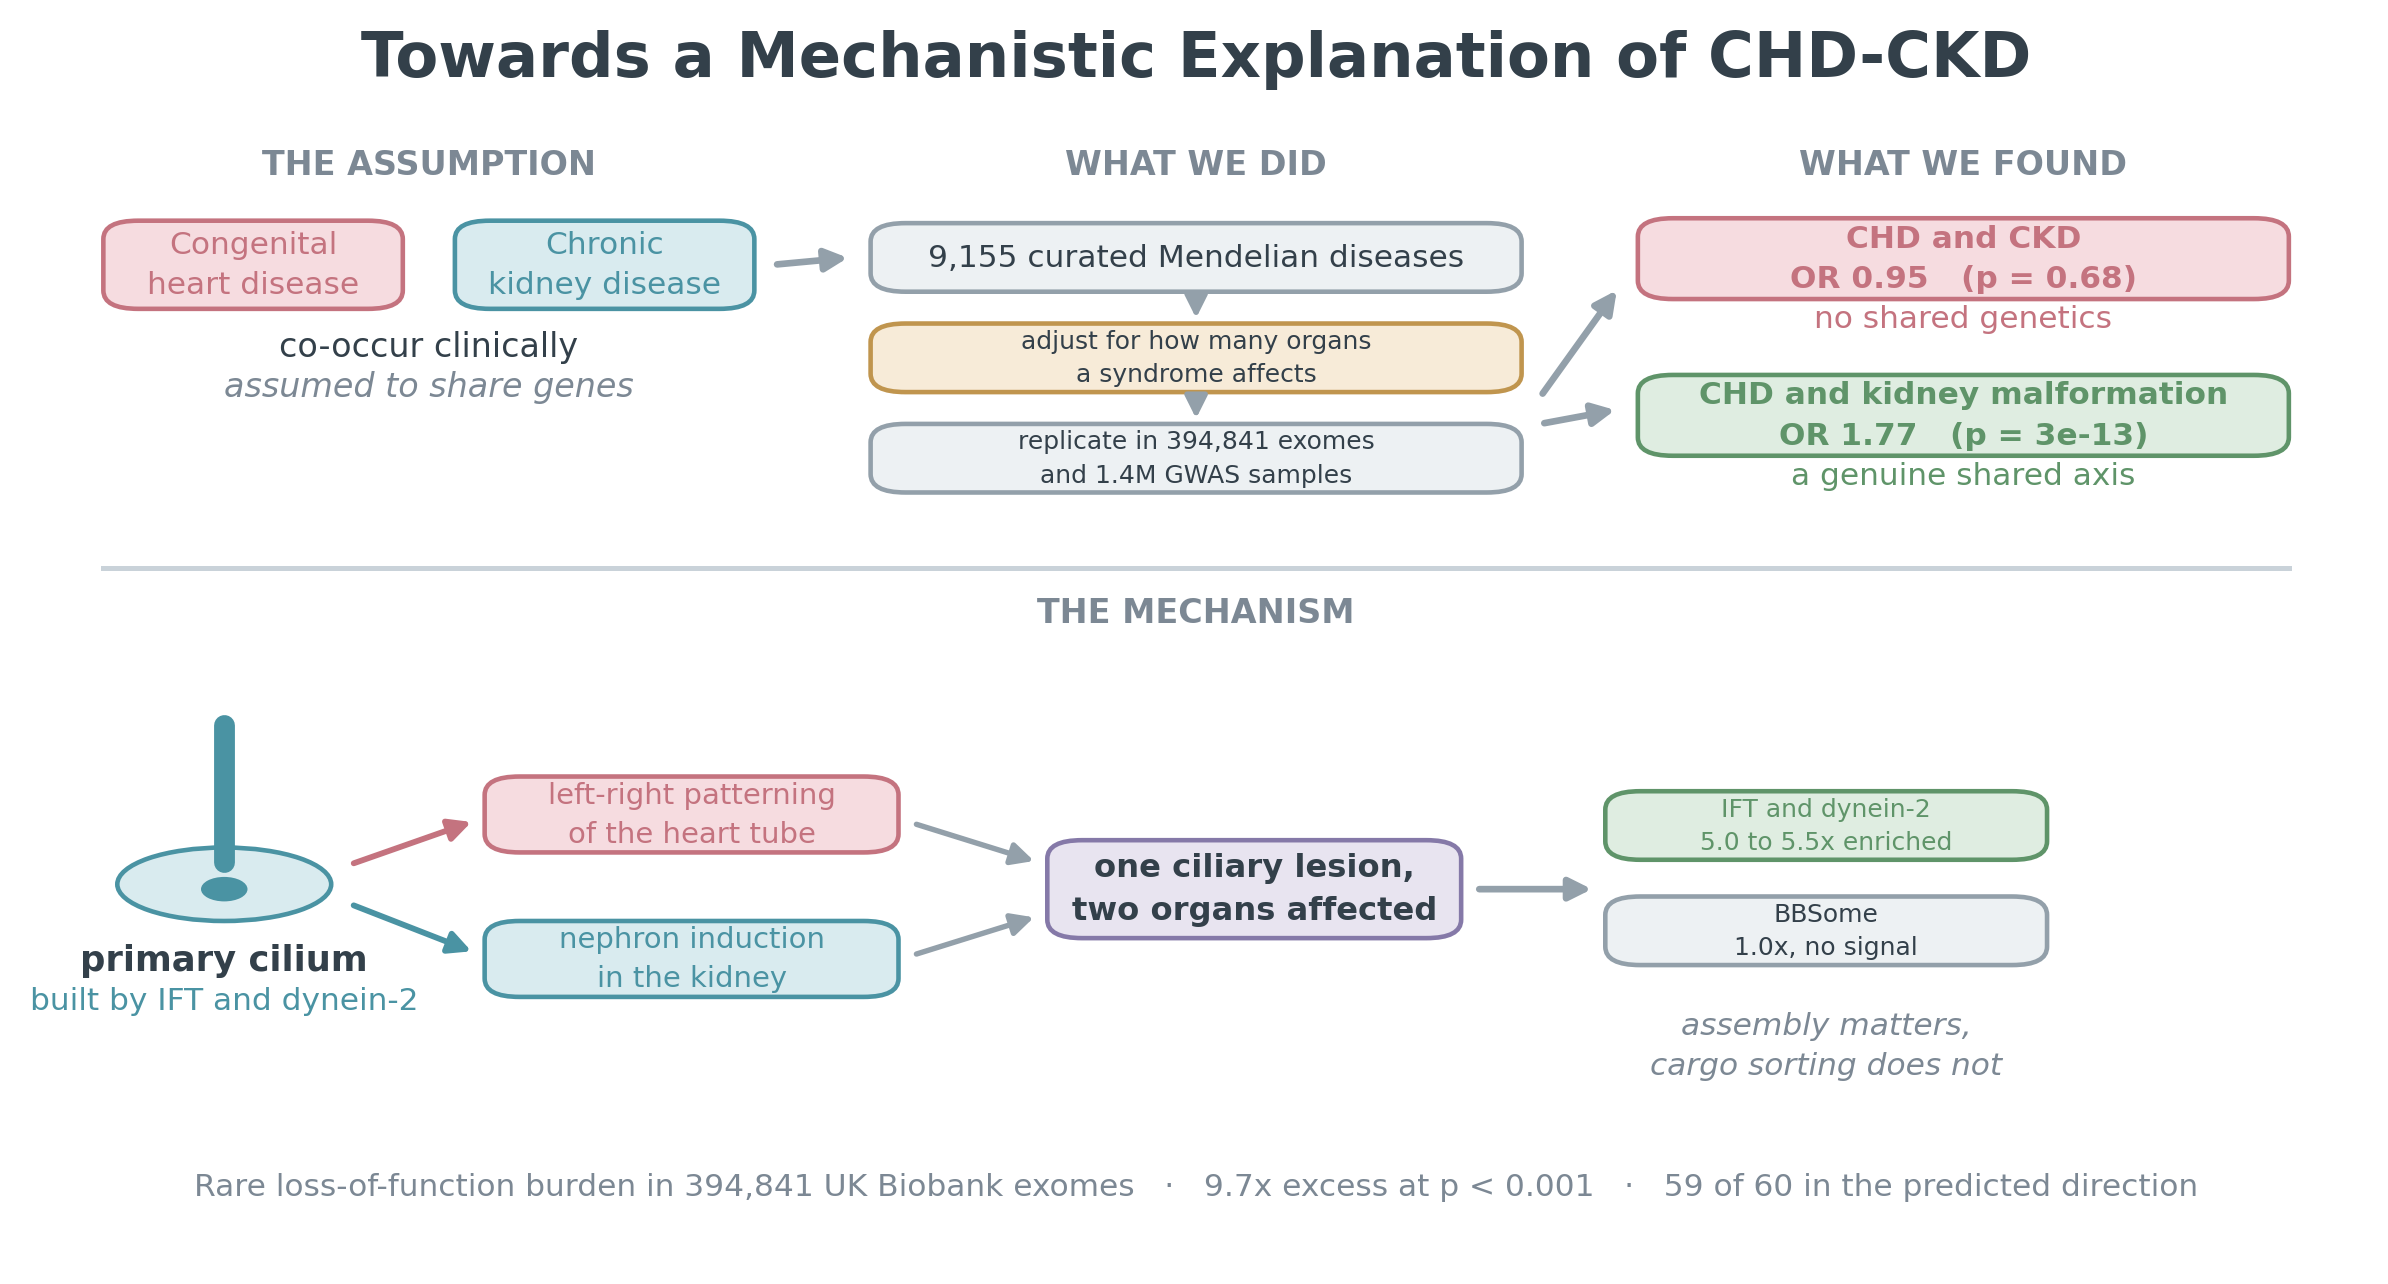
\includegraphics[width=\textwidth]{fig00_graphical_abstract.png}
\end{center}
\newpage

% ======================================================================
\section{Introduction}

Congenital heart disease is the most common congenital anomaly, affecting approximately 1\%
of live births worldwide \cite{hoffman2002,vanderlinde2011}. It encompasses a spectrum of
structural defects of the heart and great vessels, from small septal defects to complex
malformations such as hypoplastic left heart syndrome \cite{bruneau2008}. Advances in
cardiac surgery since the 1950s have transformed survival, and a growing population of
adults now lives with congenital heart disease \cite{khairy2010}.

Chronic kidney disease is a recognised comorbidity in this population. Reported prevalence
in adults with congenital heart disease is substantially higher than in the general
population \cite{morgan2015,bojan2012}, and kidney dysfunction predicts mortality in
congenital heart disease cohorts \cite{blinder2012}. Several mechanisms have been proposed:
chronic cyanosis and altered haemodynamics, repeated exposure to iodinated contrast during
catheterisation, cardiopulmonary bypass during surgical repair, and nephrotoxic medication
\cite{kumar2019,madsen2012}.

A distinct possibility is that the two conditions share genetic causes. This is biologically
plausible. The primary cilium is required both for left--right patterning during cardiac
looping and for normal nephron development, and ciliary gene defects produce syndromes
affecting both organs \cite{sanagustin2016,reiter2017}. Several Mendelian syndromes---Alagille
syndrome, the 22q11.2 deletion, Bardet--Biedl syndrome, nephronophthisis---feature cardiac and
renal involvement together.

\begin{figure}[H]
\centering
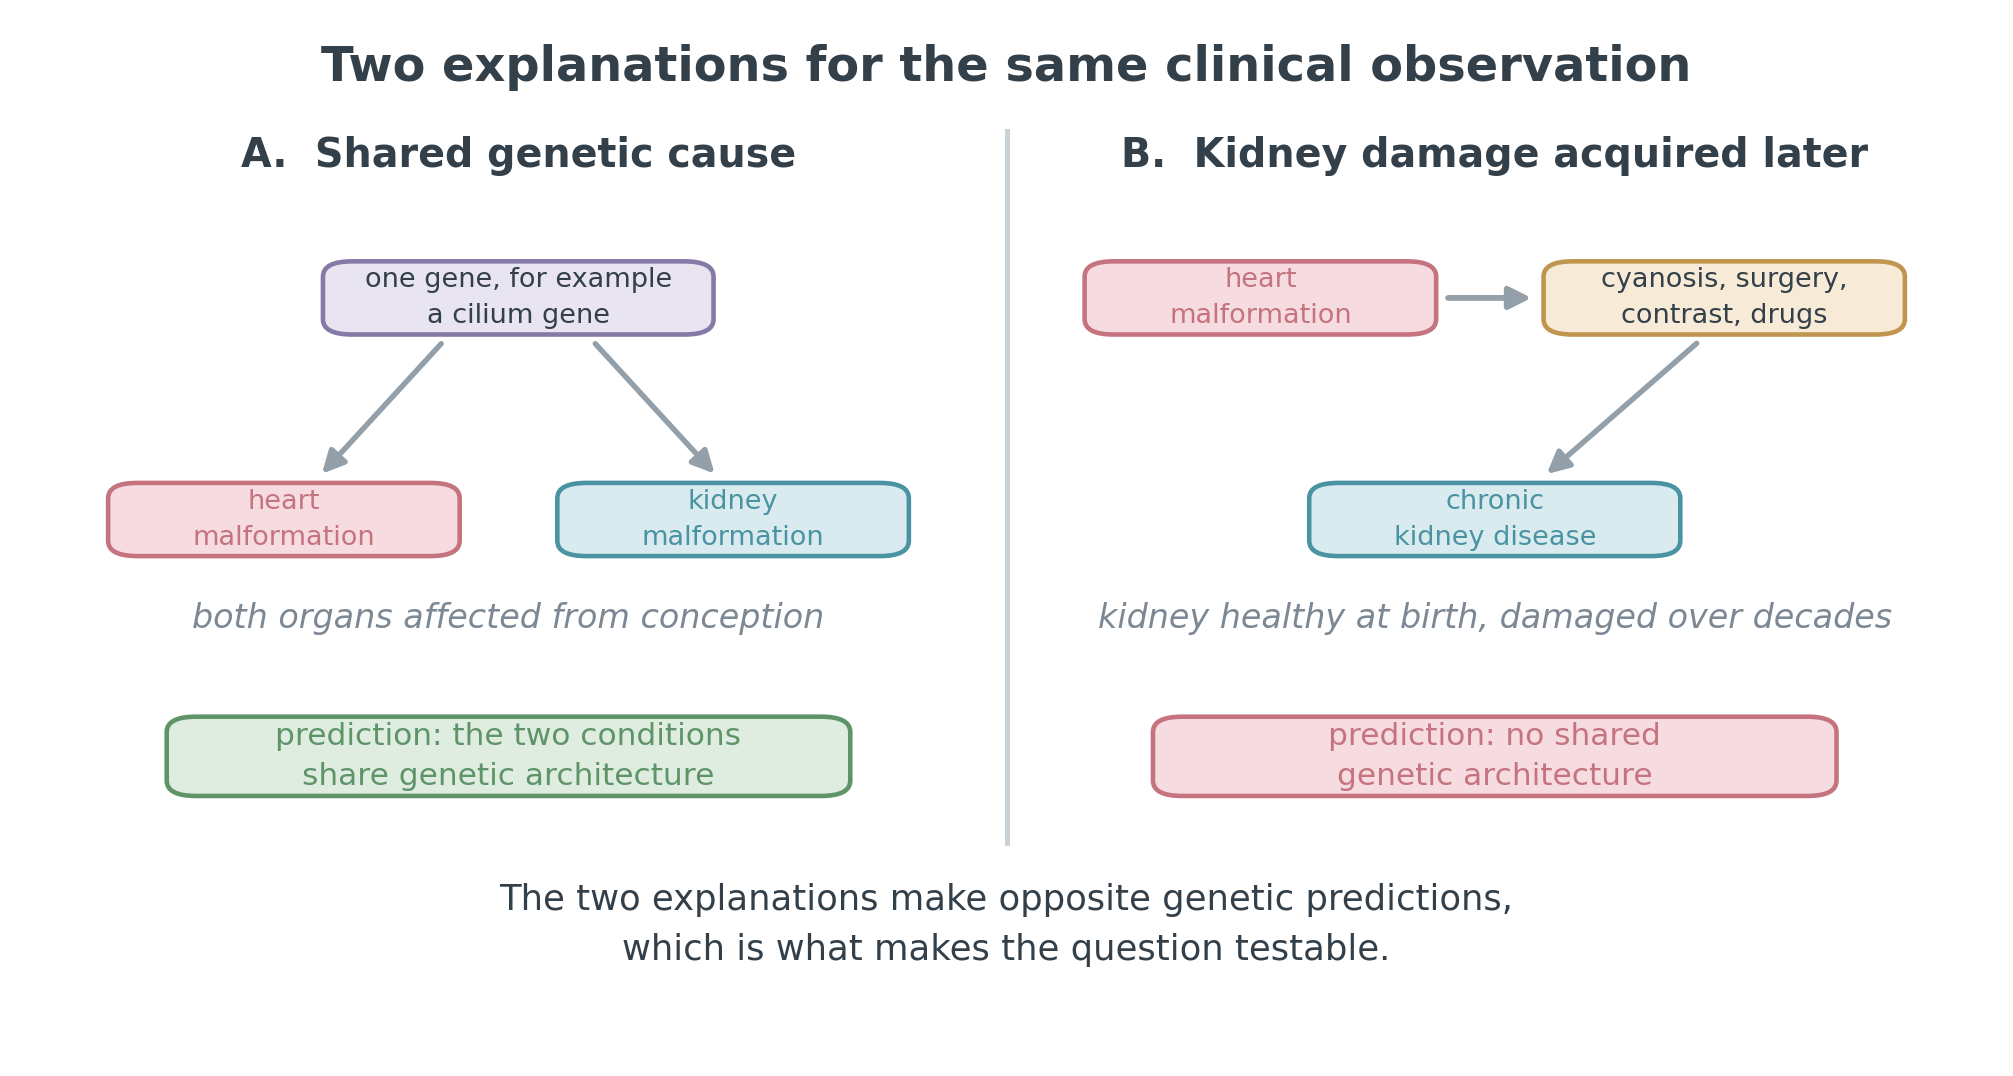
\includegraphics[width=0.92\textwidth]{figI1_two_hypotheses.png}
\caption[Two explanations for CHD--CKD co-occurrence]{Two explanations for the same
clinical observation. Under (A) a single gene disrupts both organs during development, so
the two conditions share genetic architecture. Under (B) the kidney is normal at birth and
is damaged over decades by the consequences of the cardiac lesion and its treatment. These
make opposite genetic predictions, which is what makes the question testable.}
\label{fig:hypotheses}
\end{figure}

However, plausibility is not evidence, and a specific methodological hazard applies. Genes
causing congenital malformation syndromes are typically developmental regulators that disrupt
many organs simultaneously. Any two organ systems will therefore appear to ``share'' genes
simply because syndromic genes are pleiotropic. Distinguishing a genuine cardiorenal axis from
this generic background requires an explicit control (Figure~\ref{fig:pleiotropy}).

\begin{figure}[H]
\centering
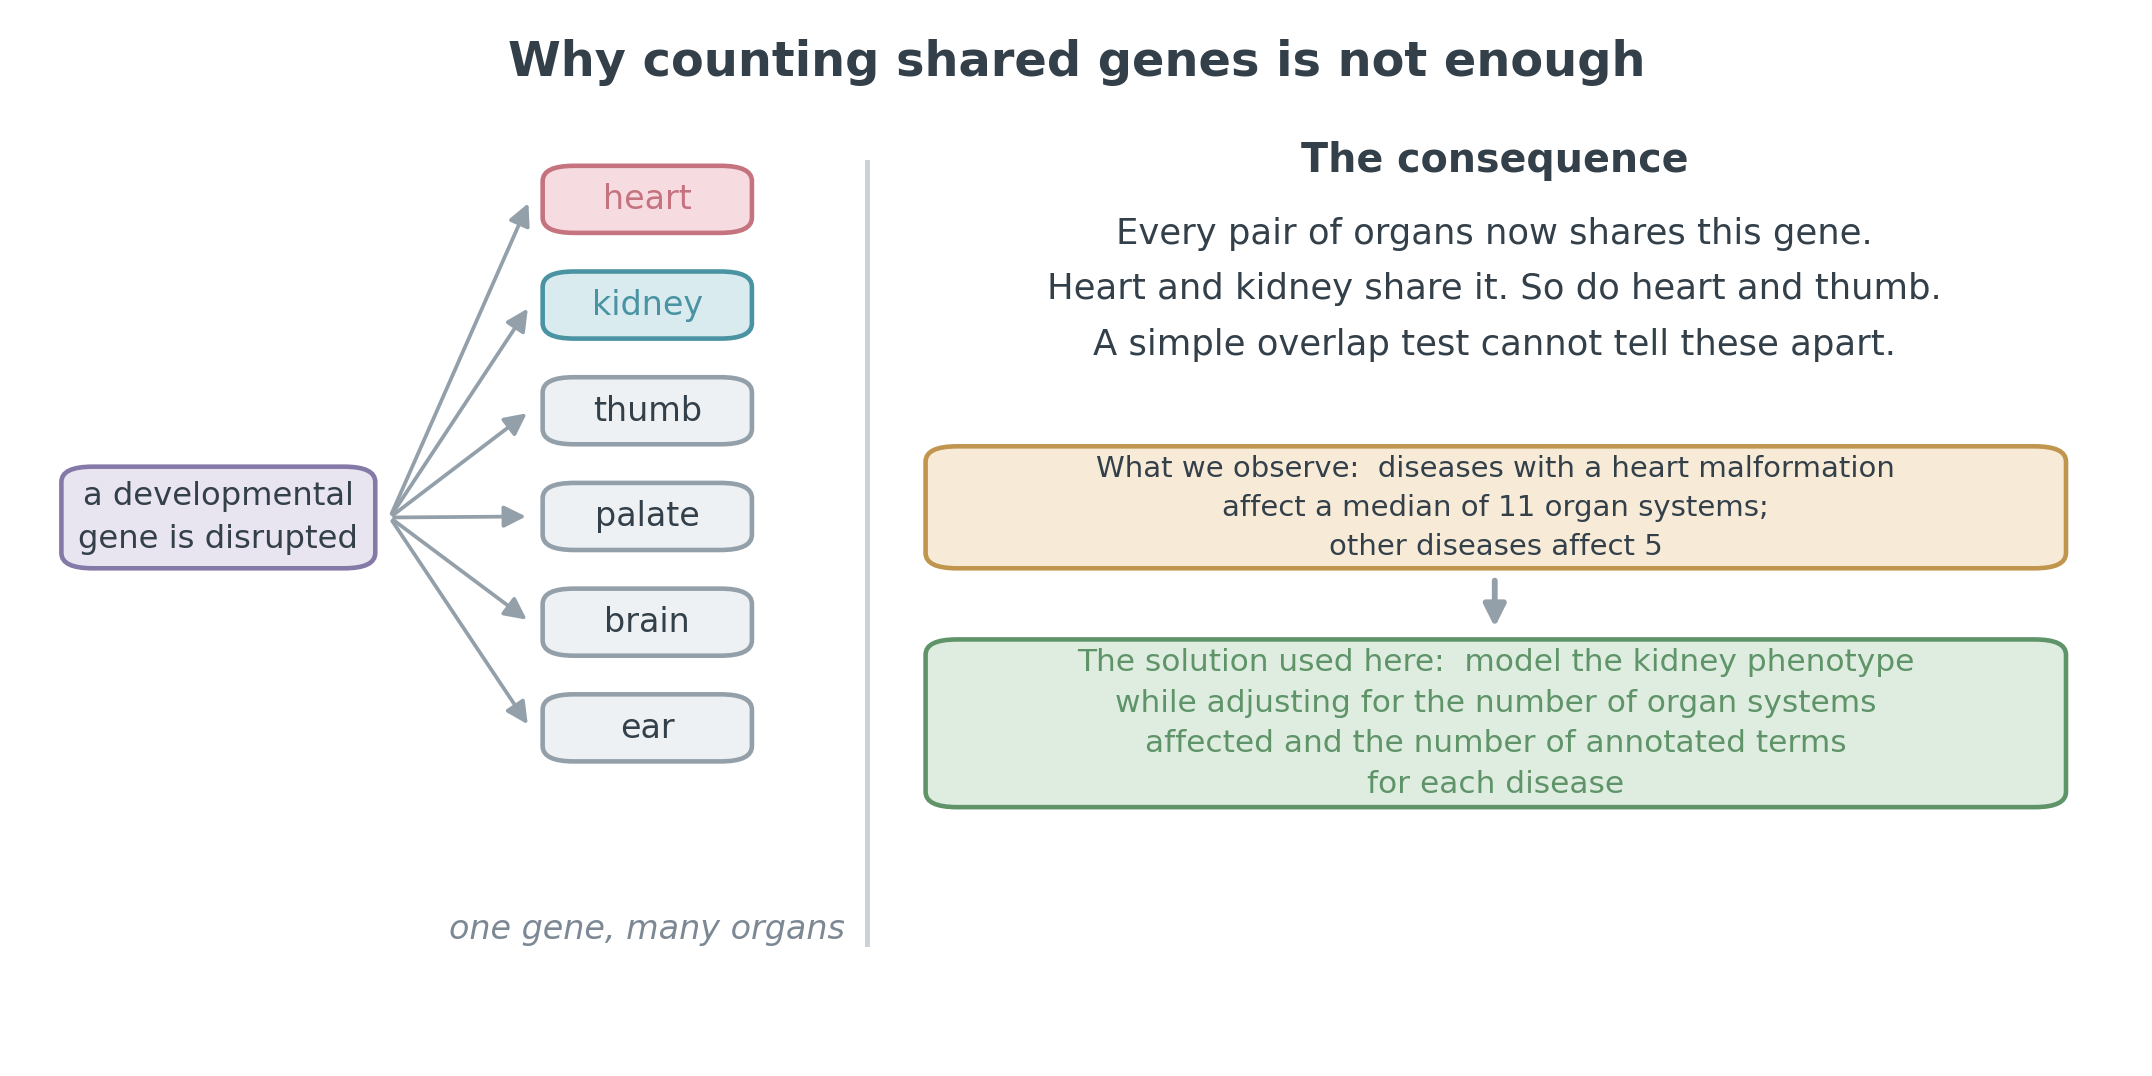
\includegraphics[width=0.92\textwidth]{figI2_pleiotropy_problem.png}
\caption[The pleiotropy problem]{Why counting shared genes is not sufficient. A gene that
disrupts early development affects many organs at once, so every pair of organs appears to
share it. A simple overlap test cannot distinguish a genuine cardiorenal relationship from
this background.}
\label{fig:pleiotropy}
\end{figure}

\subsection{Aims}

This study asked three questions:

\begin{enumerate}[leftmargin=*,itemsep=0.2em]
\item Do congenital heart disease and kidney disease share genes more than expected by
      chance, and is any such overlap specific to the kidney?
\item Does any shared signal survive adjustment for syndromic pleiotropy, and does it
      concern structural kidney malformation or chronic kidney disease as a functional
      outcome?
\item Is the conclusion reproducible in independent data using a different variant class
      and a different statistical framework?
\end{enumerate}

% ======================================================================
\section{Methodology}

All analyses used publicly available data. No individual-level genotype data were accessed,
and no ethical approval was required. The overall workflow is shown in
Figure~\ref{fig:workflow}.

\begin{figure}[H]
\centering
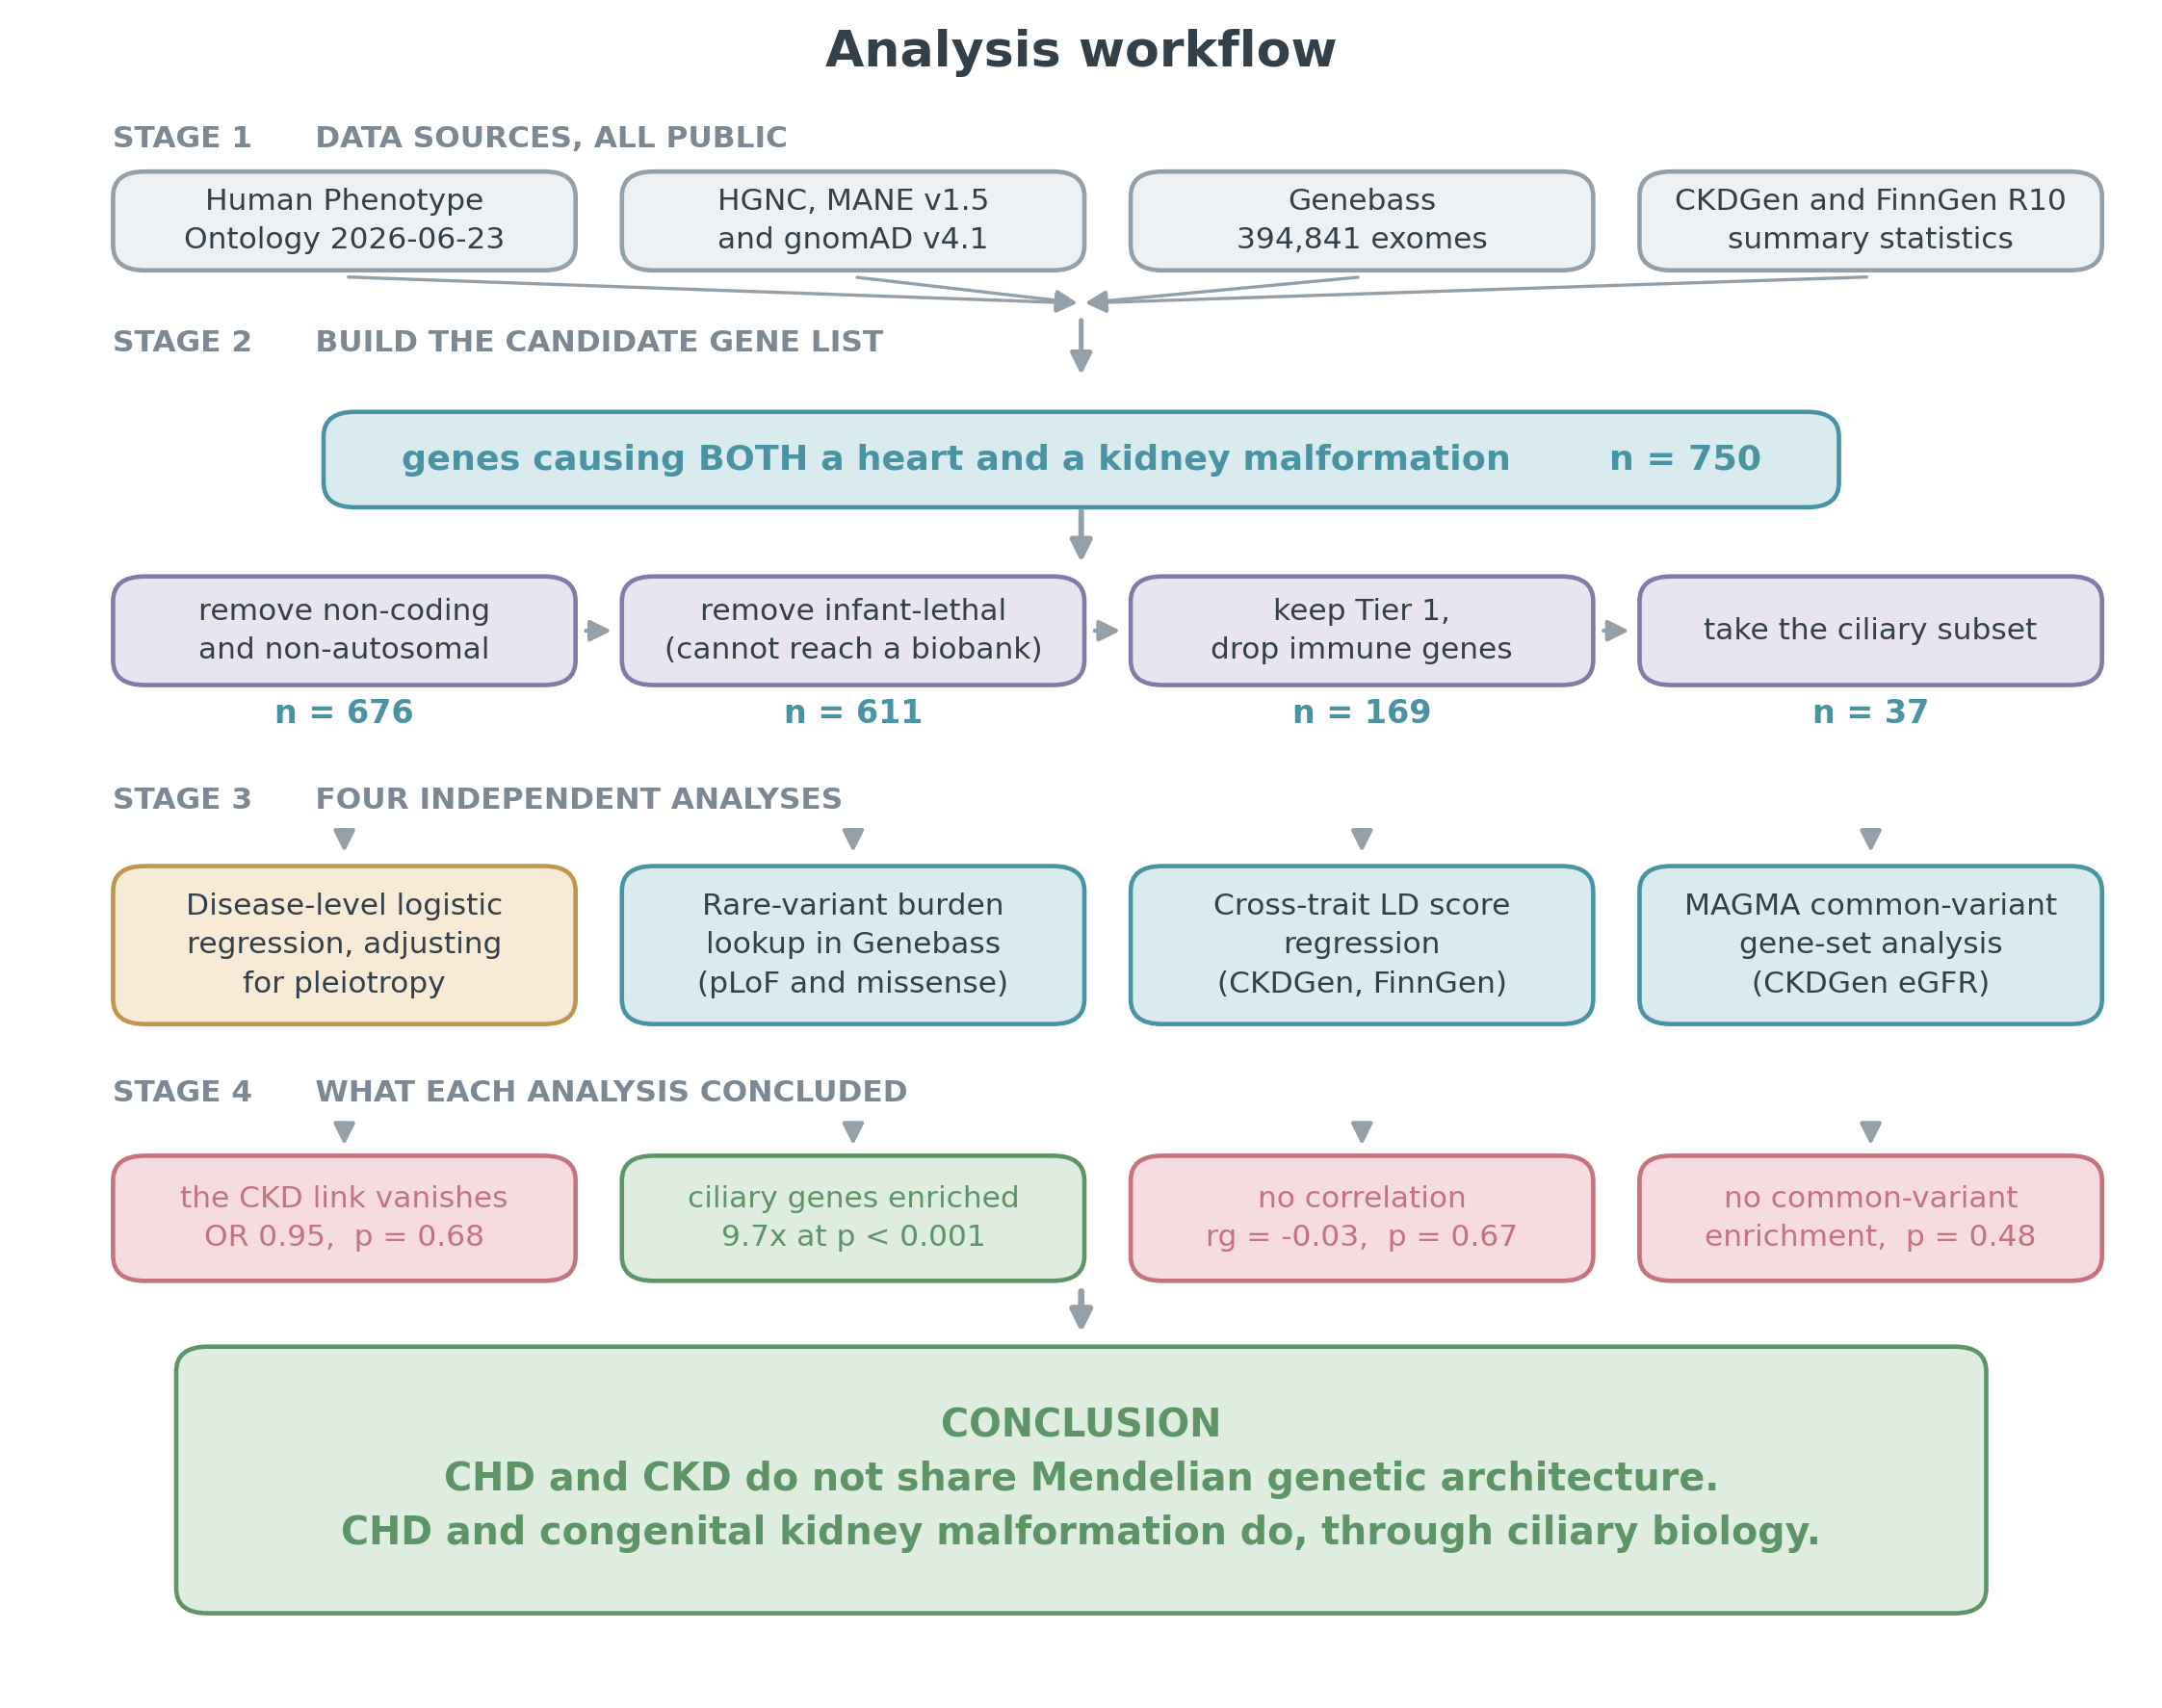
\includegraphics[width=0.95\textwidth]{figM1_workflow.png}
\caption[Analysis workflow]{Analysis workflow. Four independent analyses were applied to the
same candidate gene list: a disease-level regression controlling for pleiotropy, a
rare-variant burden lookup, cross-trait LD score regression, and a common-variant gene-set
test.}
\label{fig:workflow}
\end{figure}

\subsection{Software versions and computing environment}

All analyses were run on macOS (Darwin 25.5.0, Apple Silicon) using Python 3.9.6 with
\texttt{pandas} 1.x, \texttt{numpy}, \texttt{scipy} and \texttt{statsmodels} 0.14.6.
Figures were produced with \texttt{matplotlib} using the Agg backend at 300~dpi.
Gene-level association from summary statistics used MAGMA v1.10 \cite{deleeuw2015}.
Table~\ref{tab:versions} lists every external resource with its version and access date.

\begin{table}[H]
\centering
\small
\caption{External data resources, versions and access routes. All are public; none required
an application.}
\label{tab:versions}
\begin{tabular}{llll}
\toprule
Resource & Version / release & Content used & Access \\
\midrule
Human Phenotype Ontology & 2026-06-23 & \texttt{hp.obo}, 20,413 terms & Open (PURL) \\
HPO annotations & 2026-06-23 & 332,599 gene--phenotype rows & Open (PURL) \\
HGNC complete set & current & symbols, locus type, location & Open \\
MANE Select & v1.5 & GRCh38 gene coordinates & NCBI FTP \\
gnomAD constraint & v4.1 & pLI, LOEUF (MANE transcripts) & Google Cloud \\
Genebass & 394,841 UKB exomes & SKAT-O, burden, ACAT & Open API \\
CKDGen (Stanzick 2021) & European ancestry & eGFR, 8.84M variants & Direct download \\
FinnGen & Release 10 & CHD, CKD, cystic kidney & Direct download \\
1000 Genomes & Phase 3, EUR & LD reference for MAGMA & CTG Lab \\
LD scores & \texttt{eur\_w\_ld\_chr} & 1,290,028 HapMap 3 SNPs & Zenodo \\
MAGMA & v1.10 & gene and gene-set analysis & CTG Lab \\
\bottomrule
\end{tabular}
\end{table}

Analyses were re-run using the most recent releases of each resource available at the time
of analysis rather than the versions current when the project was first conceived; version
numbers are stated throughout so that any result can be reproduced exactly.

\subsection{Curated gene--phenotype annotations}

Gene--phenotype associations were obtained from the Human Phenotype Ontology (HPO), release
2026-06-23 \cite{gargano2024}. The ontology file (\texttt{hp.obo}, 20,413 terms) and the
gene-to-phenotype annotation file (332,599 annotations covering 5,268 genes and 9,155
diseases) were downloaded from the HPO project. These annotations derive from OMIM and
Orphanet curation rather than automated text mining, which avoids the literature-popularity
bias that affects text-mined resources.

The ontology was parsed into a directed acyclic graph and all descendant terms were resolved
for three root terms:

\begin{itemize}[leftmargin=*,itemsep=0.1em]
\item \textbf{Cardiac:} \textit{Abnormal heart morphology} (HP:0001627), 333 descendant terms
\item \textbf{Kidney (structural):} \textit{Abnormal renal morphology} (HP:0012210), 472 terms
\item \textbf{CKD (functional):} \textit{Chronic kidney disease} (HP:0012622) and
      \textit{Renal insufficiency} (HP:0000083), 15 terms combined
\end{itemize}

\subsection{Testing overlap and specificity}

Gene-set overlap was tested with a one-sided Fisher exact test against a background of all
HPO-annotated disease genes. To assess whether any overlap was specific to the kidney, the
same test was repeated against all 194 non-cardiovascular organ-morphology term sets in the
ontology containing at least 150 genes. Terms descending from
\textit{Abnormality of the cardiovascular system} (HP:0001626) were excluded to avoid
trivial self-overlap.

\subsection{Adjusting for syndromic pleiotropy}

Analysis was moved to the disease level. For each of the 9,155 diseases, binary indicators
were derived for cardiac malformation, structural kidney anomaly and CKD, together with two
measures of pleiotropy: the number of the 23 top-level HPO organ systems affected, and the
total number of annotated terms. Logistic regression was then fitted:

\begin{equation}
\mathrm{logit}\,P(\text{kidney phenotype}) = \beta_0 + \beta_1 \cdot \text{CHD}
 + \beta_2 \cdot n_{\text{systems}} + \beta_3 \cdot n_{\text{terms}}
\end{equation}

where $\exp(\beta_1)$ is the adjusted odds ratio of interest. The same model was fitted
separately for each of twelve specific cardiac lesions.

\subsection{Candidate gene list construction}

Genes annotated to both a cardiac and a kidney malformation term were retained (750 genes),
then annotated with current approved symbols, chromosomal location and locus type from HGNC
\cite{seal2023}, genomic coordinates from MANE Select v1.5 \cite{morales2022}, and
loss-of-function constraint (pLI and LOEUF) from gnomAD v4.1 \cite{chen2024}. Non-coding and
non-autosomal genes were removed.

A survivability filter was then applied. Genes whose only documented phenotypes included
perinatal or infant lethality (HP:0001522, HP:0003811, HP:0003826, HP:0034241, HP:0003819)
with no adult- or juvenile-onset disease on record were excluded, because affected
individuals cannot appear in an adult cohort. This removed 65 genes, leaving 611.

Genes were then tiered by whether they additionally had documented CKD or renal
insufficiency. Tier 1 (178 genes) required all three. Immune-mediated genes entering through
autoimmune disease (HLA loci, \gene{PTPN22}, \gene{STAT4}, \gene{MEFV}, \gene{IL6},
\gene{IL10}, \gene{TLR4}, \gene{HFE}, \gene{SAA1}, \gene{TNXB}) were removed as
mechanistically distinct, giving 169 genes. A 37-gene ciliary subset was defined from the
ciliopathy, nephronophthisis and polycystic kidney disease mechanism classes. Six of these
are already established causes of cystic kidney disease (\gene{PKD1}, \gene{PKD2},
\gene{IFT140}, \gene{ALG9}, \gene{GANAB}, \gene{DNAJB11}); because including them in a
pooled test would guarantee a positive result that merely rediscovers autosomal dominant
polycystic kidney disease, they were held out as a positive control and the remaining 31
genes pre-specified as the primary set. Figure~\ref{fig:funnel} summarises the filtering.

\begin{figure}[H]
\centering
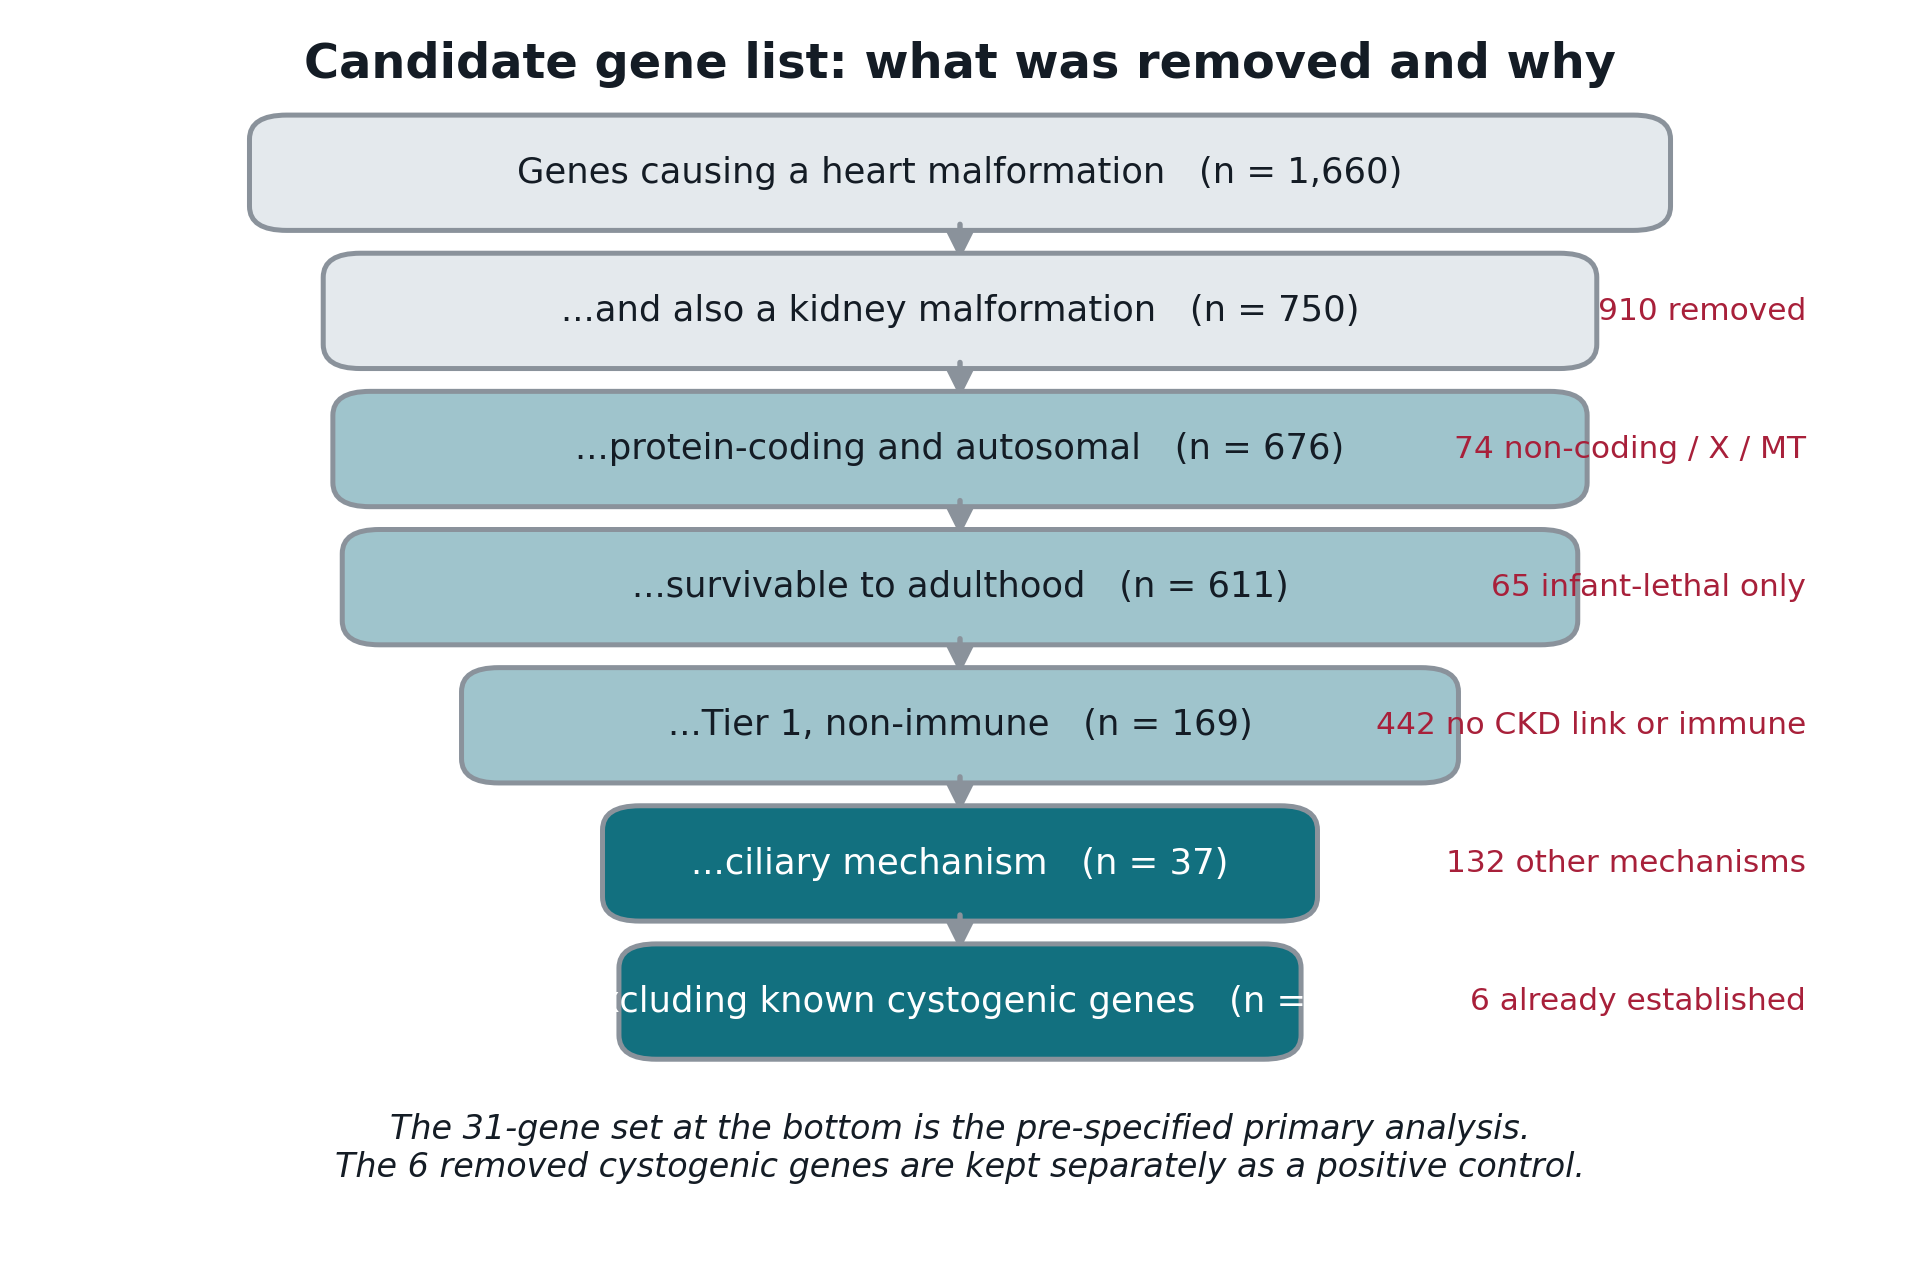
\includegraphics[width=0.88\textwidth]{figM2_gene_filtering.png}
\caption[Gene list filtering]{Construction of the candidate gene list, showing how many
genes were removed at each step and why. Bar widths are proportional to
$\log_{10}(n)$.}
\label{fig:funnel}
\end{figure}

\subsection{Gene burden statistics from exome sequencing}

Rare-variant gene-burden association statistics were obtained from Genebass
\cite{karczewski2022}, which provides SKAT-O \cite{lee2014}, burden and ACAT
\cite{liu2019} tests across 4,529 phenotypes in 394,841 UK Biobank exomes
\cite{bycroft2018,szustakowski2021}. Results were retrieved programmatically for each
candidate gene and filtered to twenty renal phenotypes: five continuous biomarkers
(creatinine, cystatin C, urea, microalbumin, urinary creatinine) and fifteen ICD-10 based
endpoints. Both the predicted loss-of-function (pLoF) and missense burden sets were
retrieved, the latter serving as a negative control.

Enrichment was assessed by comparing observed counts of nominally significant results against
the number expected under the null. Because individual genes were underpowered, a
directional test was also applied: among results with $p < 0.05$, the proportion with a
positive effect estimate (worse kidney function) was compared against 0.5 with an exact
binomial test. Under the null this proportion is 0.5 regardless of selection on $p$.

\subsection{Cross-trait LD score regression}

Genetic correlation was estimated by cross-trait LD score regression
\cite{bulik2015a,bulik2015b}. Summary statistics were obtained for estimated glomerular
filtration rate from CKDGen (European-ancestry meta-analysis, 8.8 million variants,
mean $n = 980{,}825$) \cite{stanzick2021}, and for congenital malformations of the heart and
great arteries (4,270 cases), chronic kidney disease (10,039 cases) and cystic kidney disease
(947 cases) from FinnGen release 10 \cite{kurki2023}.

Variants were restricted to the HapMap 3 subset used for the pre-computed European LD scores
(1,290,028 SNPs, $M_{5,50} = 1{,}173{,}569$) derived from 1000 Genomes Phase 3
\cite{1000g2015}. Strand-ambiguous variants, those with minor allele frequency below 0.01,
and those with $\chi^2 > \max(80, 0.001N)$ were removed. Effective sample size
$N_{\text{eff}} = 4/(1/n_{\text{case}} + 1/n_{\text{control}})$ was used for binary traits.

Heritability was estimated from the regression
$\mathbb{E}[\chi^2_j] = 1 + (Nh^2/M)\ell_j$, and genetic covariance from
$\mathbb{E}[z_{1j}z_{2j}] = (\sqrt{N_1N_2}\,\rho_g/M)\ell_j + a$, where the intercept $a$
absorbs sample overlap. Standard errors came from a 200-block genome-ordered jackknife.
Because the reference implementation requires Python 2, which no longer installs cleanly, the
estimator was reimplemented; it was validated against a published heritability estimate and
against a positive control trait pair before the results below were interpreted.

\subsection{Common-variant gene and gene-set analysis}

Gene-level association was computed with MAGMA v1.10 \cite{deleeuw2015} from the CKDGen
European-ancestry eGFR meta-analysis. SNP identifiers, chromosomes and build-37 positions
were extracted for all 8,842,706 variants carrying an rs identifier. SNPs were assigned to
genes using the NCBI37.3 gene location file with a zero-kilobase window, so only variants
within the transcribed region contribute; 18,038 of 19,427 genes received at least one SNP.
Gene $p$-values used the default SNP-wise mean model with the 1000 Genomes Phase 3 European
panel (503 individuals) as LD reference.

Gene-set analysis used MAGMA's competitive test, which asks whether genes in a set have
smaller $p$-values than genes outside it, conditioning internally on gene size, gene
density, sample size and minor allele count together with the logarithms of each. Four sets
were tested: all 37 ciliary genes, the 31 with cystogenic genes removed, the 6 cystogenic
genes alone, and the 166 Tier 1 genes with a gene-location entry. Gene symbols were mapped
to Entrez identifiers through HGNC; all four sets mapped completely.

\subsection{Multiple testing}

Three correction strategies were used, chosen to match each question.

For the HPO organ-specificity screen (194 tests) and the disease-level regressions, results
are reported with exact confidence intervals and $p$-values without correction, because the
comparison of interest is between two pre-specified models rather than a search across many.

For the gene-burden lookups, two thresholds are quoted: Bonferroni across the tests
performed ($0.05/706 = 7.1\times10^{-5}$ for the ciliary set,
$0.05/3226 = 1.5\times10^{-5}$ for Tier 1), and the conventional exome-wide threshold for
gene-based tests of $2.5\times10^{-6}$. Benjamini--Hochberg $q$-values
\cite{benjamini1995} are additionally reported. The Benjamini--Hochberg step-up procedure is
implemented as $q_{(i)} = \min_{j \geq i}\left(\frac{n}{j}p_{(j)}\right)$, evaluated by a
cumulative minimum running from the largest $p$-value downwards; the implementation was
checked against \texttt{statsmodels.stats.multitest}.

For the MAGMA gene-set analysis, four sets were tested and no result survives Bonferroni
correction at $0.05/4 = 0.0125$.

\subsection{Directional testing}

Because individual genes in the candidate set are underpowered, a test with greater
sensitivity was applied. Among gene $\times$ phenotype results with $p < 0.05$, the
proportion with a positive burden effect (indicating worse kidney function) was compared
against 0.5 with an exact binomial test. This is valid despite selection on $p$: under the
null hypothesis the sign of an effect estimate is independent of its magnitude, so selected
results remain equally likely to point either way. An empirical null was also constructed by
drawing 200,000 samples from $\mathrm{Binomial}(n, 0.5)$ to confirm the analytic $p$-value.

\subsection{Reproducibility}

All analysis code is available at \texttt{github.com/sahoo2000/chd-ckd-genetics}, organised
as numbered scripts to be run in order. Every result table and figure in this report is
regenerated by that code from the public sources in Table~\ref{tab:versions}. Intermediate
result files are included in the repository so that figures can be redrawn without
repeating the slow steps; the MAGMA gene analysis in particular takes approximately four
hours.

% ======================================================================
\section{Results}

\subsection{Cardiac and kidney genes overlap, but not specifically}

Of the genes with curated disease annotations, 1,660 cause a cardiac malformation and 1,198
cause a kidney malformation. The 750-gene overlap is far beyond chance (OR 5.81,
$p = 1.5 \times 10^{-144}$).

This overlap is not specific to the kidney. Repeating the identical test against 194
non-cardiovascular organ systems placed the kidney only 16th (Figure~\ref{fig:organs}). The
median odds ratio across all organ systems was 3.76, so the kidney sits only 1.5 times above
a typical organ. Thumb (6.36), uvula (6.49), soft palate (6.80) and abdominal wall (6.53)
morphology all overlap cardiac genes more strongly than the kidney does.

\begin{figure}[H]
\centering
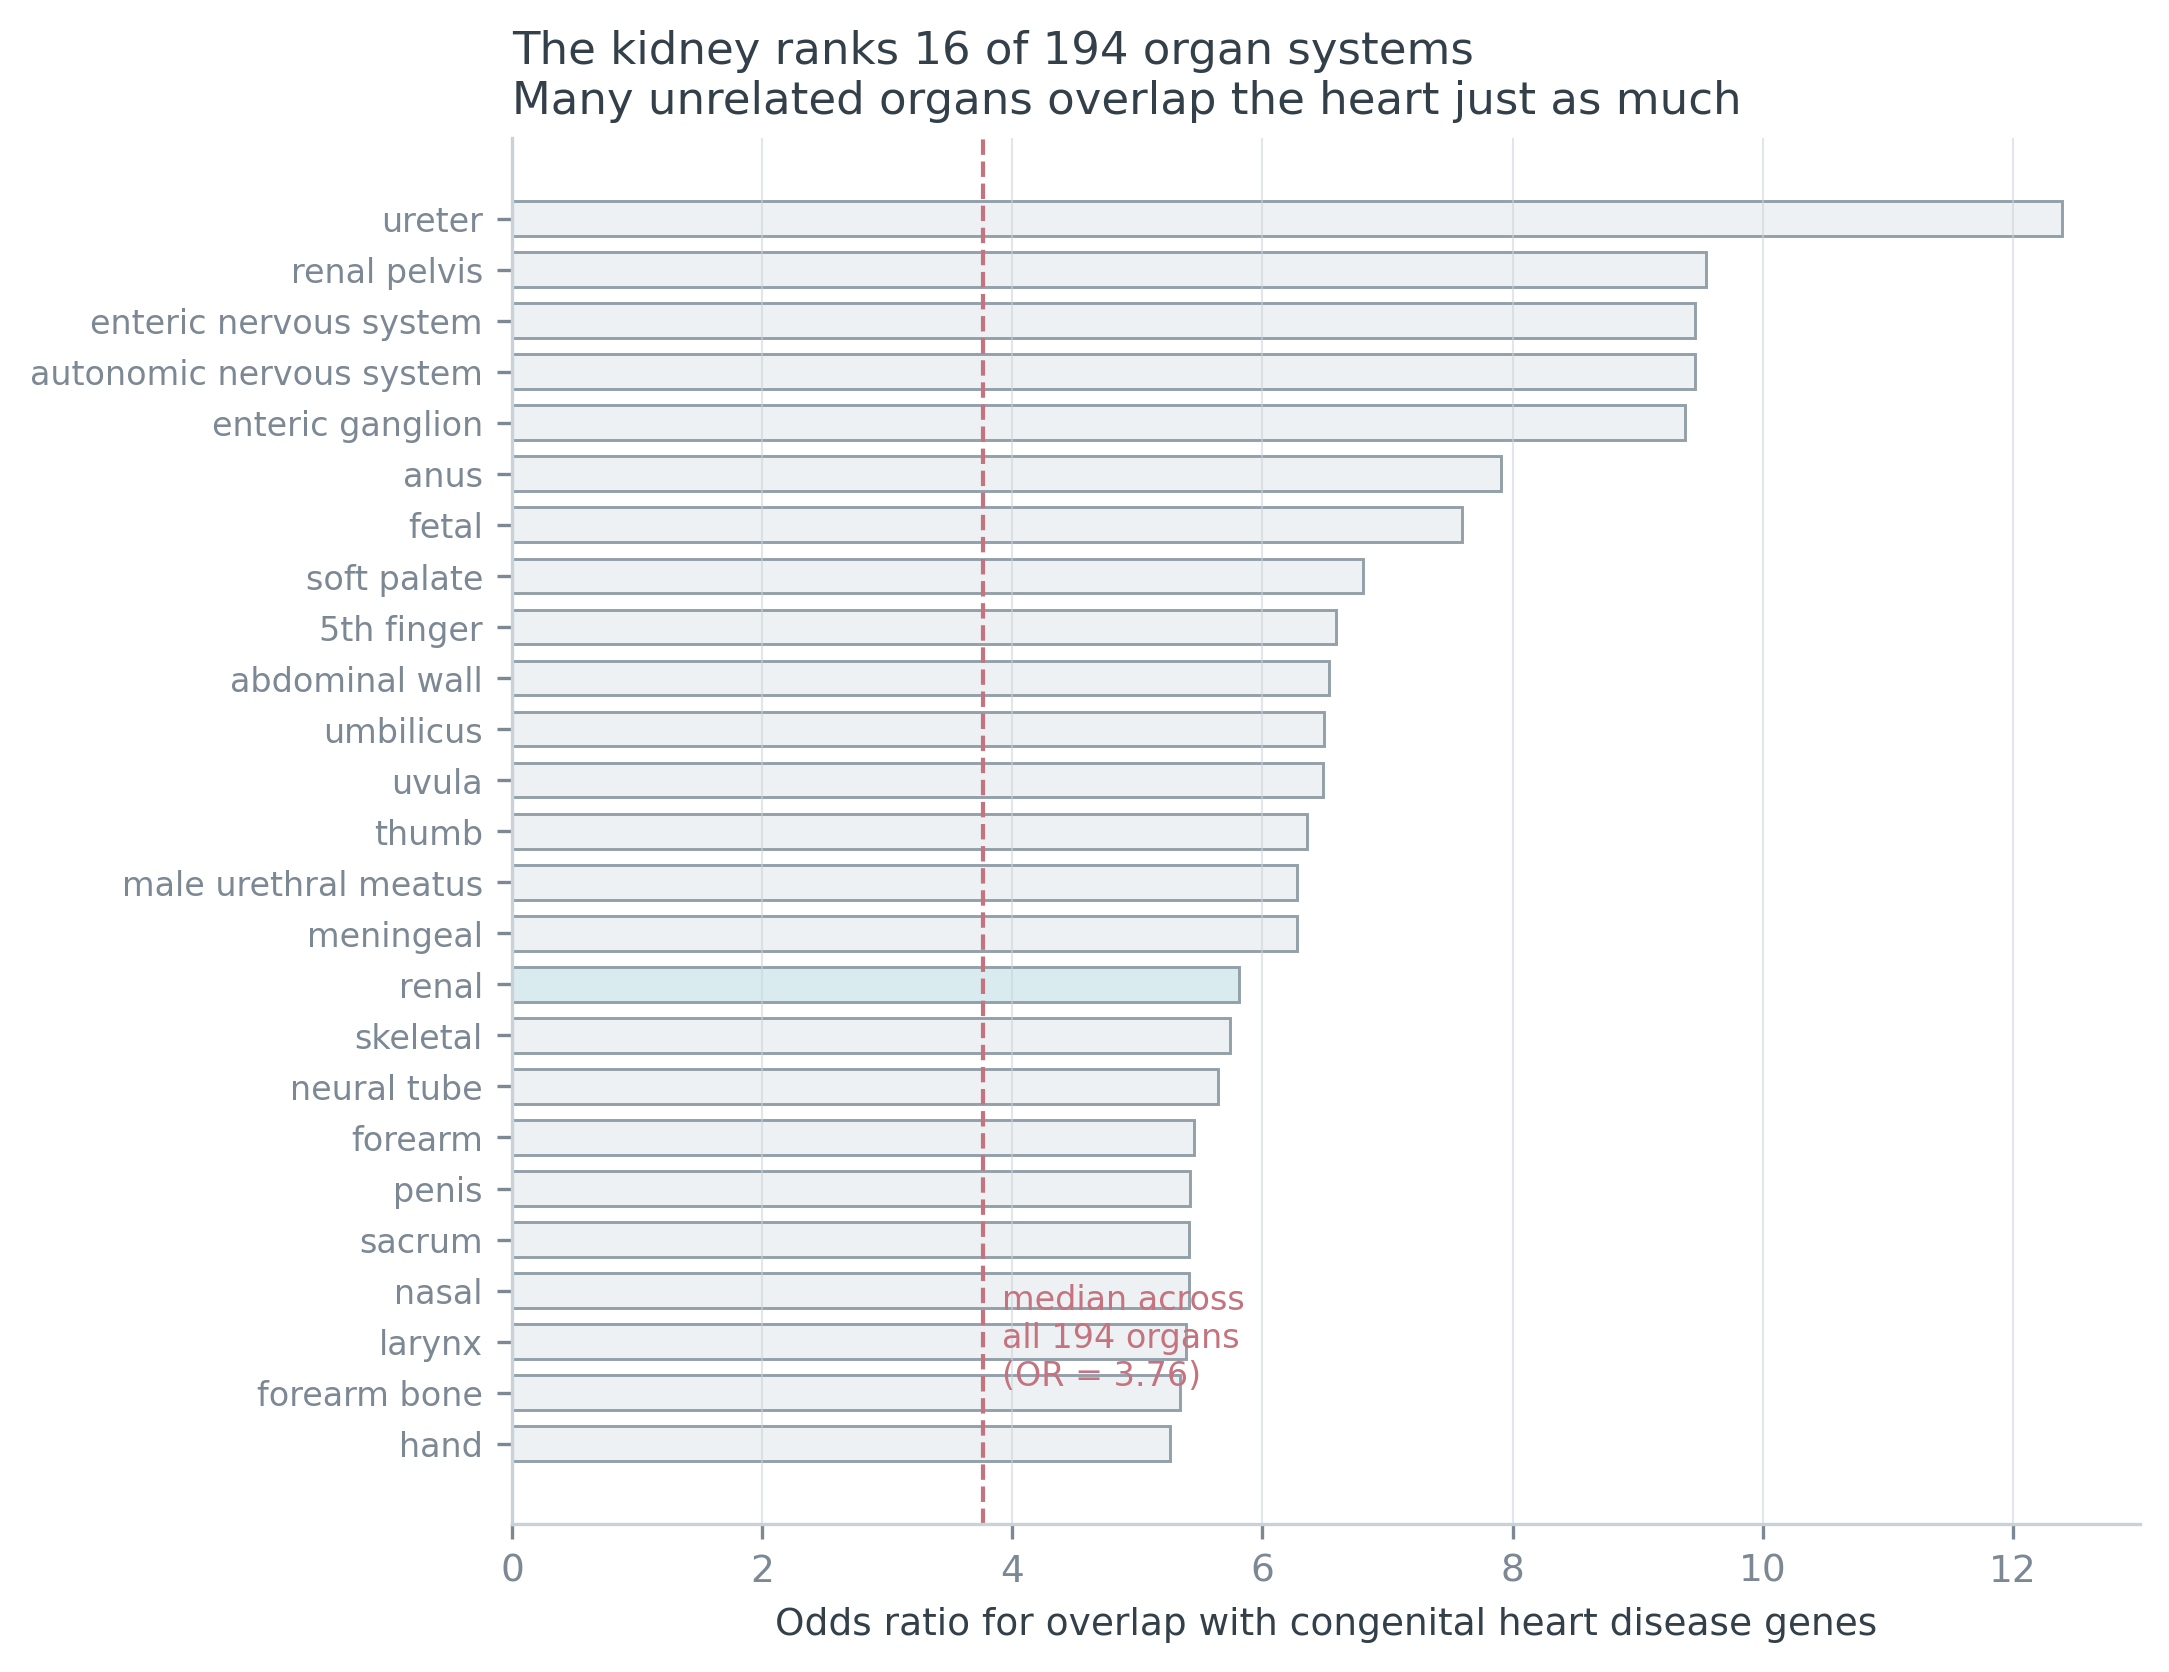
\includegraphics[width=0.86\textwidth]{fig02_organ_specificity.png}
\caption{Overlap of congenital heart disease genes with each organ system. The kidney
(highlighted) ranks 16th of 194. Many anatomically unrelated structures overlap the heart as
strongly, which is the signature of syndromic pleiotropy rather than a specific
cardiorenal axis.}
\label{fig:organs}
\end{figure}

The explanation is pleiotropy. Diseases involving a cardiac malformation affect a median of
11 organ systems, against 5 for all other diseases (Mann--Whitney $p = 5.3 \times
10^{-297}$). Genes disrupting early development disrupt many organs at once.

\subsection{Adjustment separates two different questions}

After adjusting for the number of organ systems affected and the number of annotated terms,
the two putative associations behave completely differently (Figure~\ref{fig:forest};
Table~\ref{tab:forest}).

\begin{table}[H]
\centering
\small
\caption{Disease-level association between congenital heart disease and kidney phenotypes,
before and after adjustment for pleiotropy ($n = 9{,}155$ diseases).}
\label{tab:forest}
\begin{tabular}{lcccc}
\toprule
Outcome & Model & OR & 95\% CI & $p$ \\
\midrule
Structural kidney anomaly & Unadjusted & 4.21 & 3.69--4.81 & $2.0\times10^{-94}$ \\
Structural kidney anomaly & Adjusted   & 1.77 & 1.52--2.07 & $3.1\times10^{-13}$ \\
Chronic kidney disease    & Unadjusted & 1.57 & 1.25--1.97 & $1.3\times10^{-4}$ \\
Chronic kidney disease    & Adjusted   & 0.95 & 0.73--1.23 & 0.68 \\
\bottomrule
\end{tabular}
\end{table}

\begin{figure}[H]
\centering
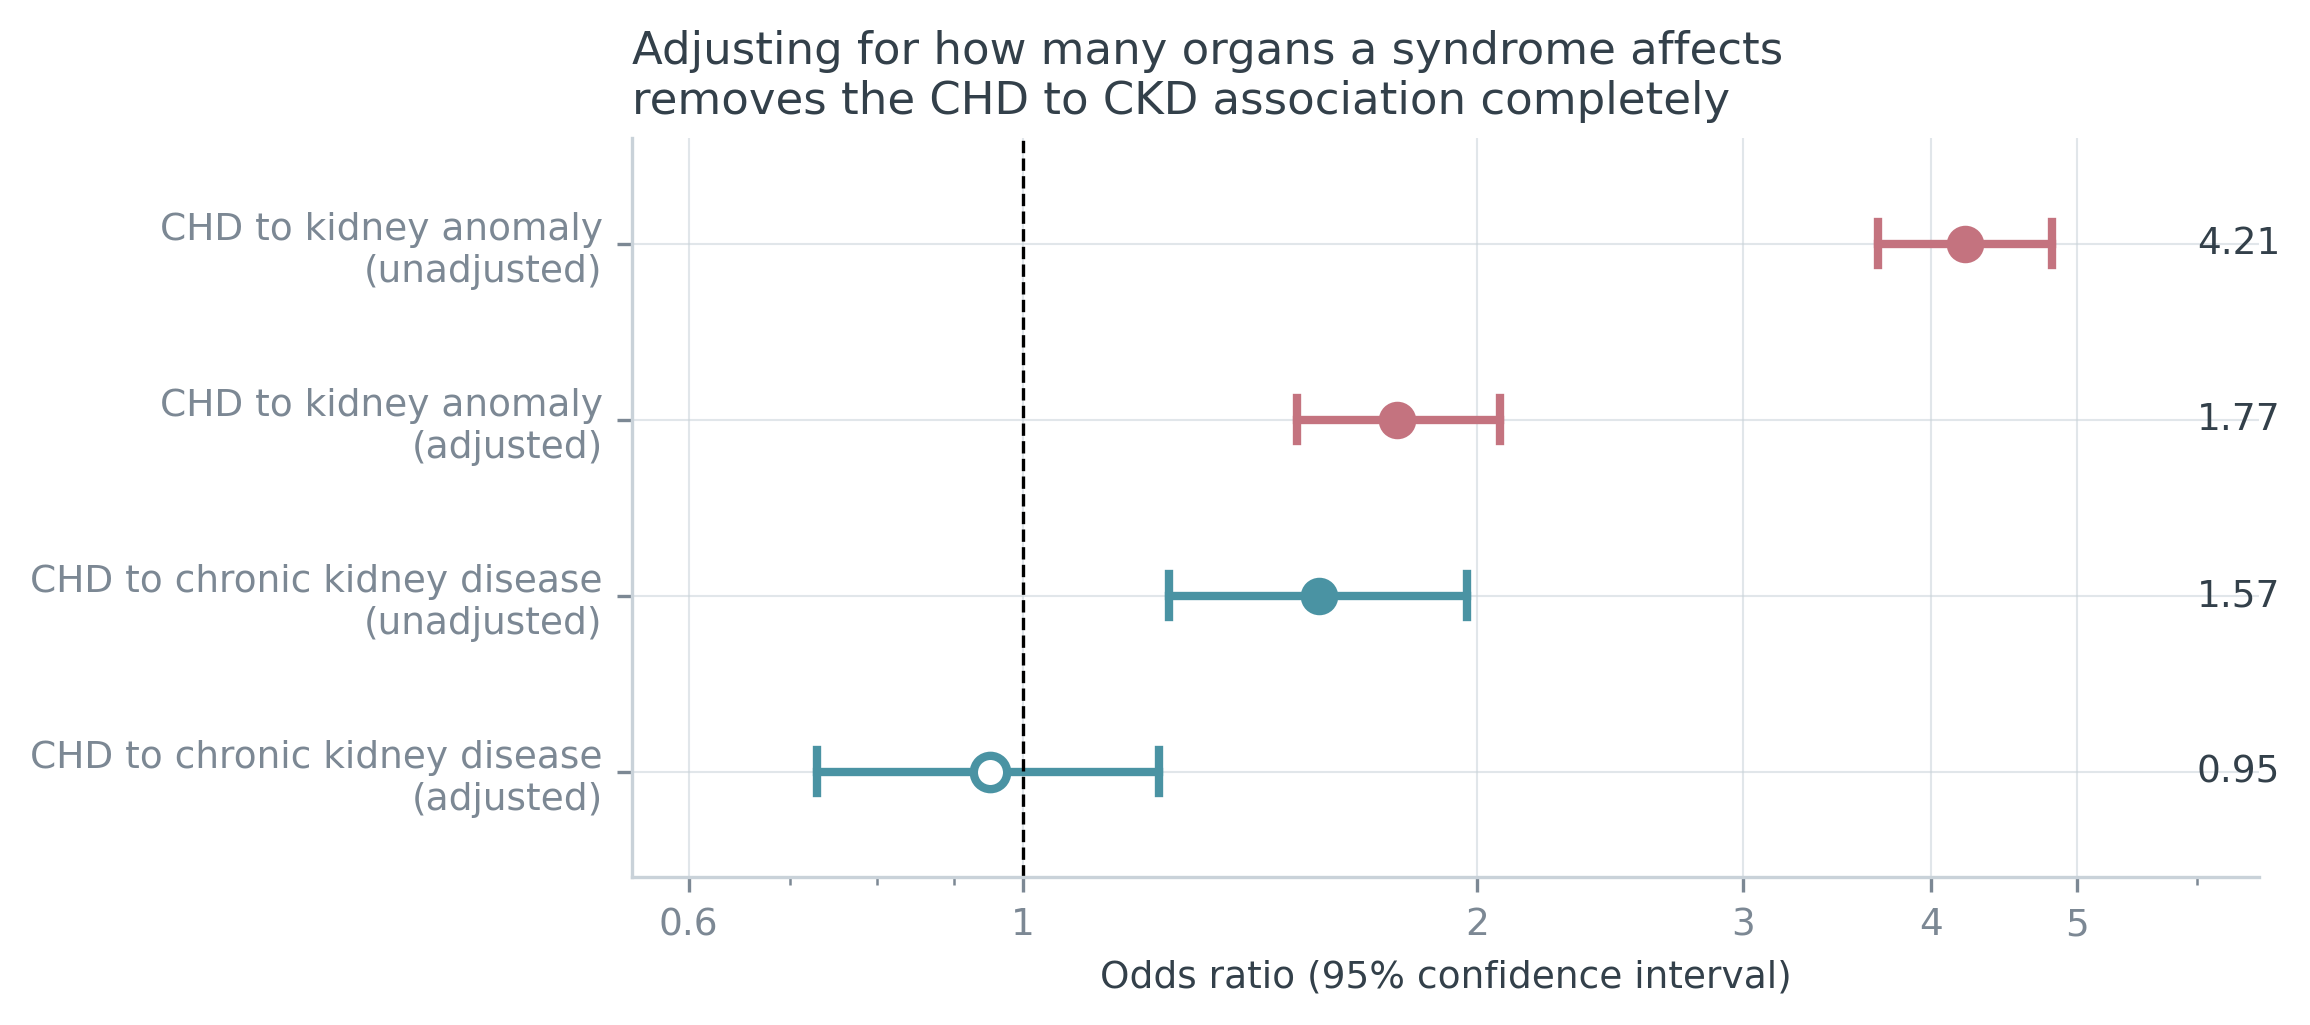
\includegraphics[width=0.9\textwidth]{fig01_forest_adjusted_odds_ratios.png}
\caption{Odds ratios with 95\% confidence intervals. The association with structural kidney
malformation survives adjustment; the association with chronic kidney disease does not, and
its adjusted interval spans the null.}
\label{fig:forest}
\end{figure}

The association with structural kidney malformation is attenuated but robust. The association
with chronic kidney disease disappears entirely: the naive odds ratio of 1.57 is fully
explained by the fact that heart-malformation syndromes affect many organs.

\subsection{The lesions carrying the signal are absent from adult cohorts}

Testing each cardiac lesion separately (Figure~\ref{fig:lesions}) showed that the strongest
associations with kidney anomaly come from hypoplastic left heart syndrome (adjusted OR 6.13,
95\% CI 3.24--11.6), tetralogy of Fallot (4.83, 3.15--7.41) and atrioventricular canal defect
(2.22, 1.29--3.82). These are precisely the lesions that an adult cohort recruited at ages
40--69 will barely contain. The lesions that such a cohort does contain in numbers---bicuspid
aortic valve (1.89), pulmonic stenosis (1.77), atrial septal defect (2.13)---sit at the bottom
of the ranking.

\begin{figure}[H]
\centering
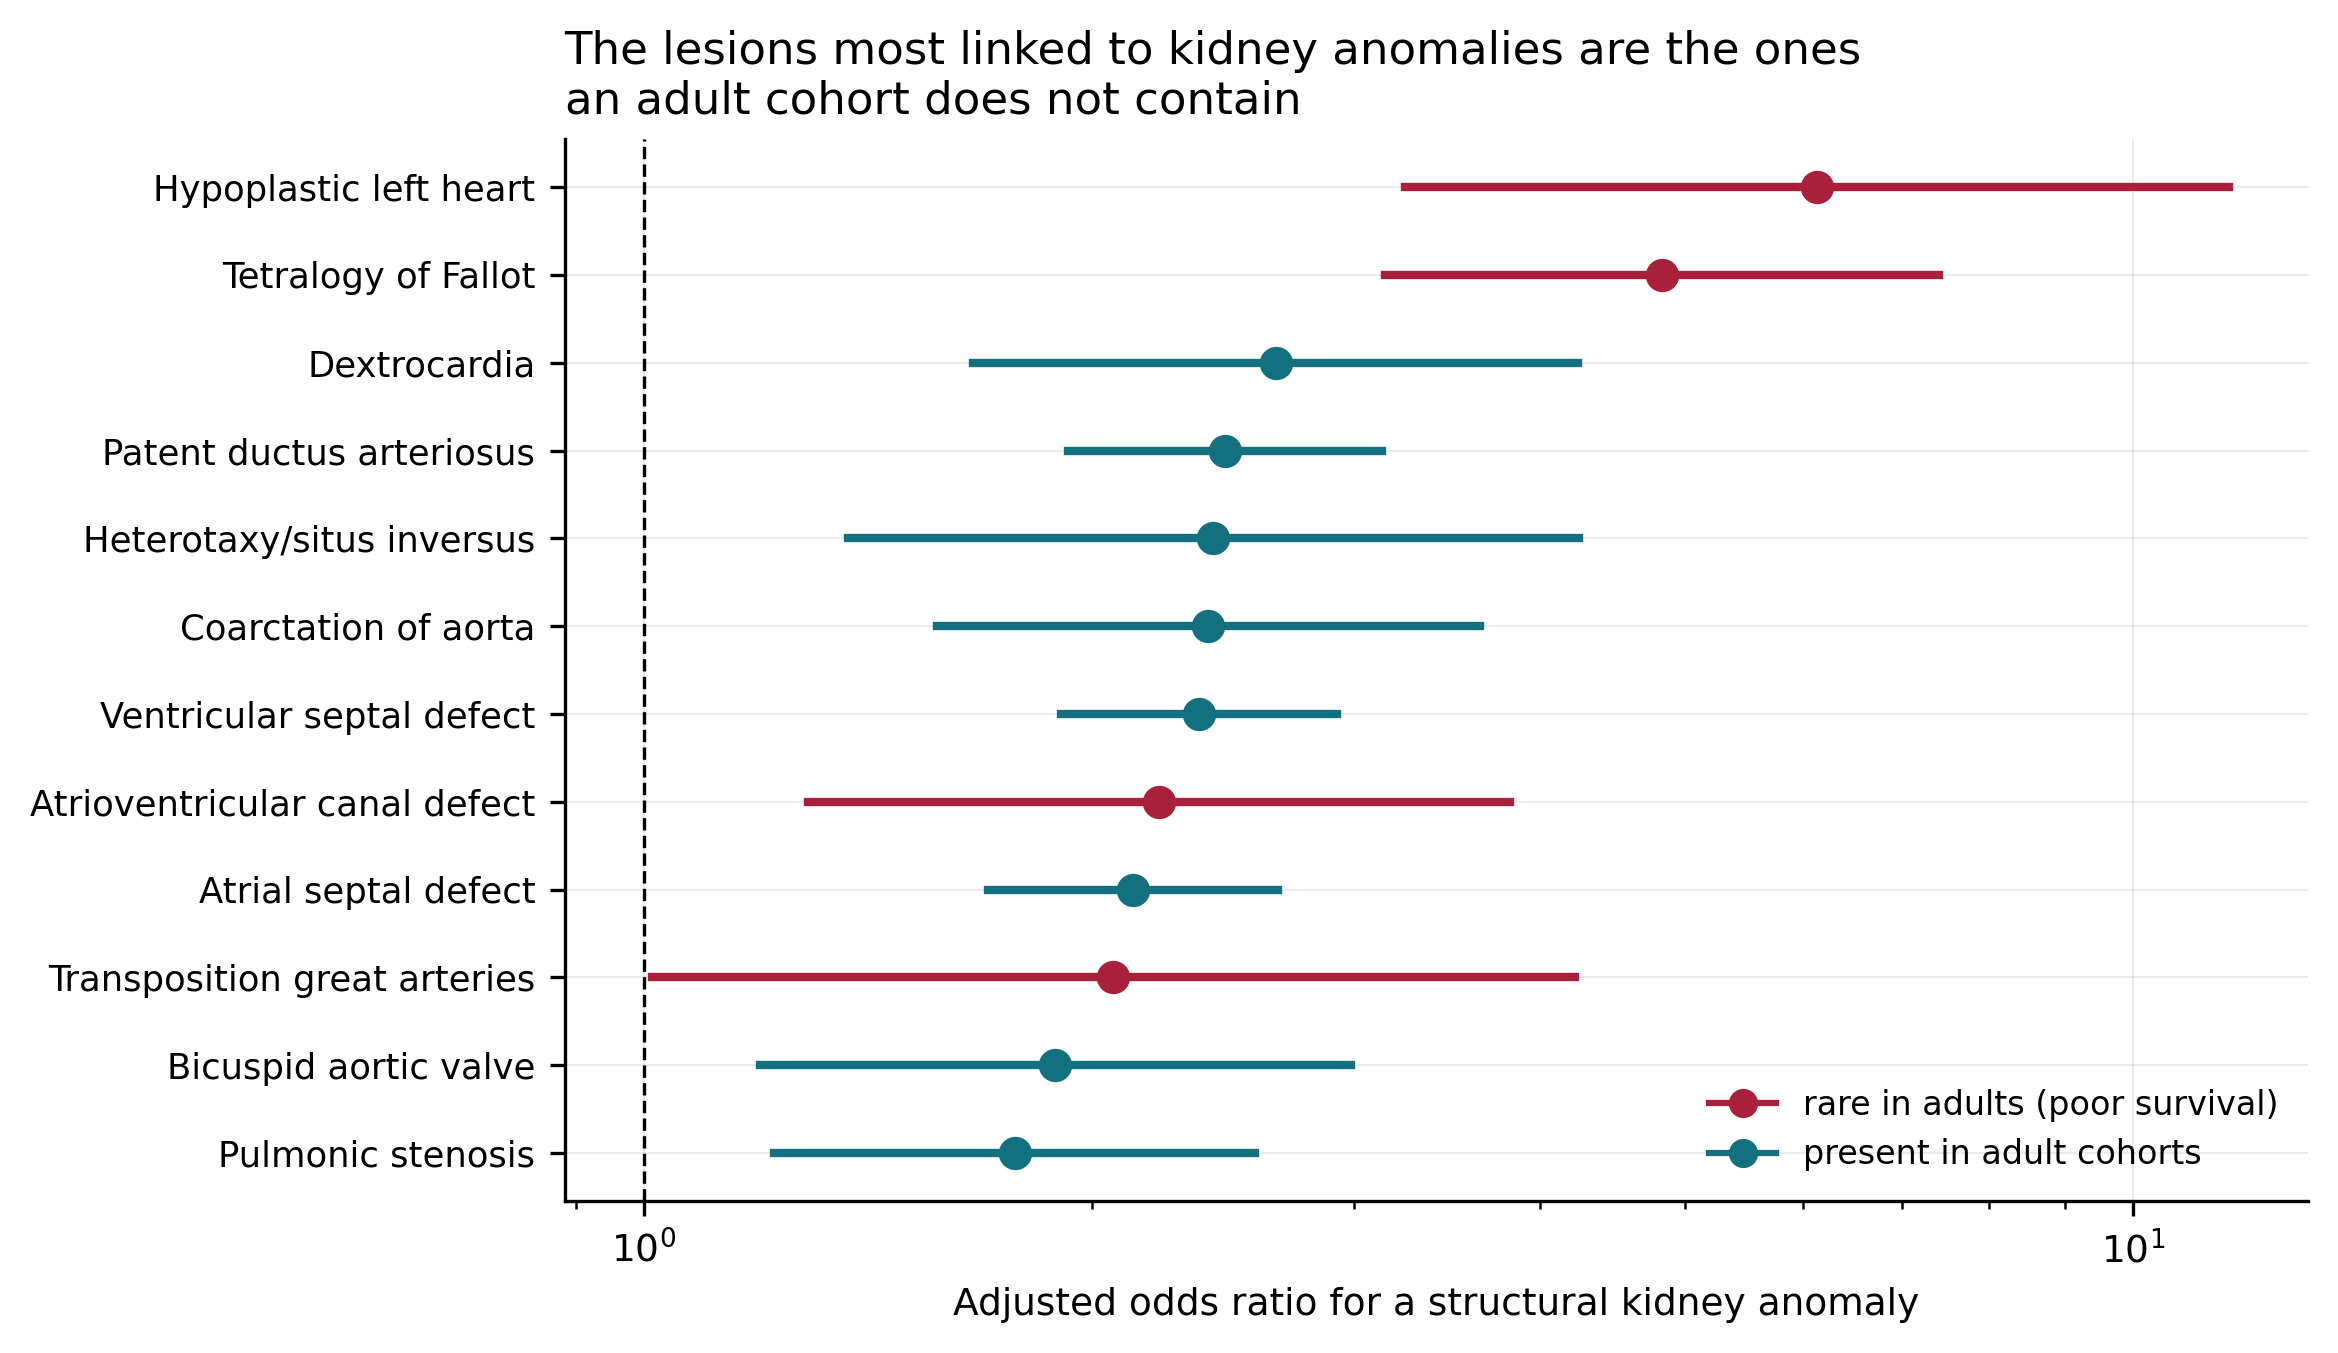
\includegraphics[width=0.9\textwidth]{fig03_lesion_odds_ratios.png}
\caption{Adjusted odds ratio for a structural kidney anomaly, by cardiac lesion. The ordering
runs almost exactly opposite to availability in an adult biobank.}
\label{fig:lesions}
\end{figure}

This has a direct consequence for study design. In UK Biobank there are approximately 3,385
congenital heart disease cases and 1,386 cases of congenital kidney anomaly among roughly
450,000 participants. If independent, about 10 individuals would carry both; applying the
observed enrichment gives roughly 18 (Figure~\ref{fig:samplesizes}). No burden test has power
on 18 cases at any effect size. A continuous kidney measurement, by contrast, is available in
376,624 participants.

\begin{figure}[H]
\centering
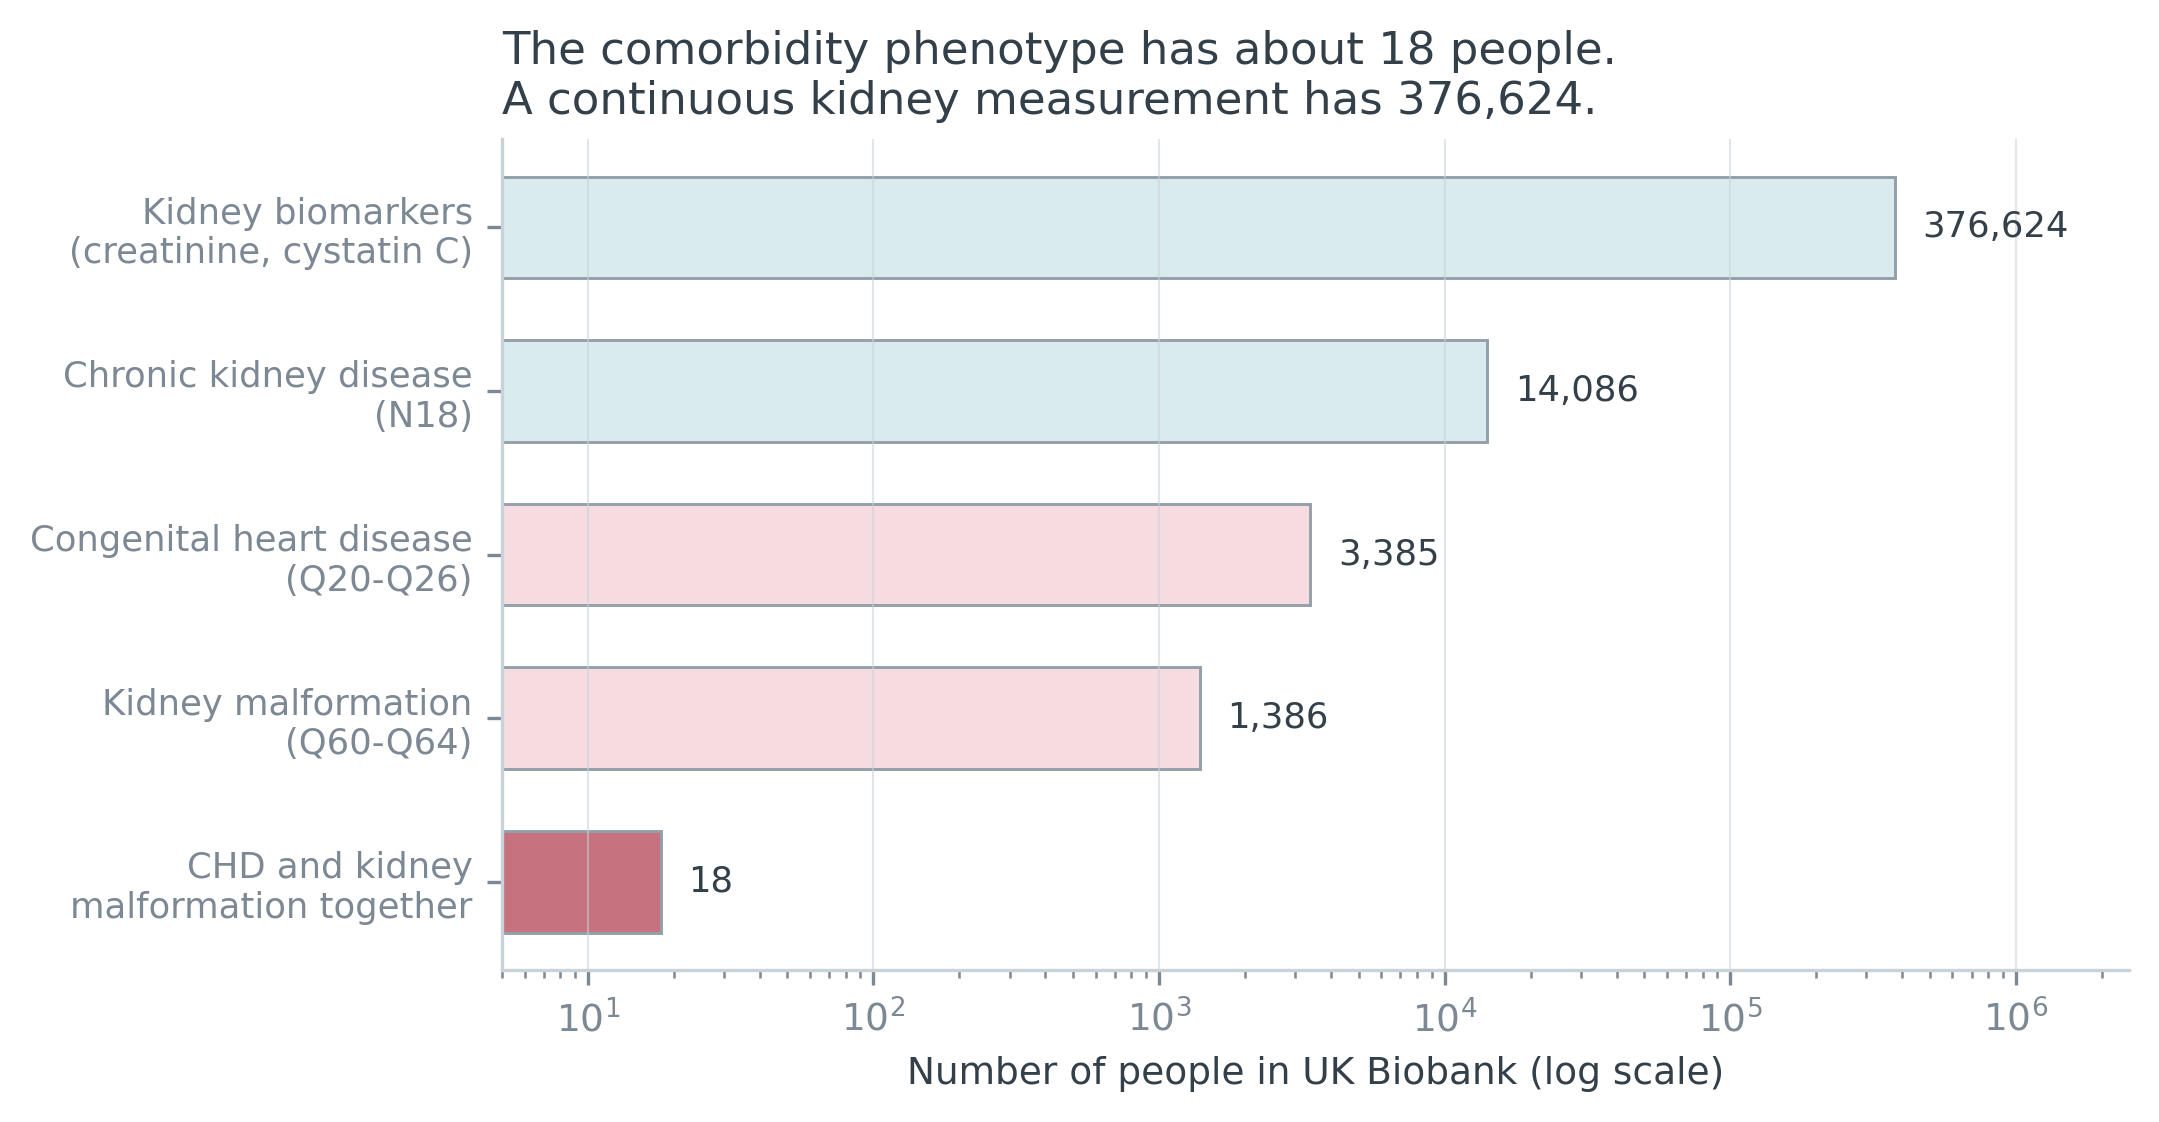
\includegraphics[width=0.85\textwidth]{fig09_sample_sizes.png}
\caption{Available sample sizes in UK Biobank. The comorbidity phenotype is not analysable;
a quantitative kidney trait is measured in essentially everyone.}
\label{fig:samplesizes}
\end{figure}

\subsection{Independent replication in 394,841 exomes}

Gene-burden statistics were retrieved for 165 Tier 1 genes, giving 3,226 gene $\times$ renal
phenotype associations. Four genes reach exome-wide significance ($p < 2.5 \times 10^{-6}$),
and all four are dominant, adult-onset cystogenic genes (Table~\ref{tab:genebass};
Figure~\ref{fig:volcano}). The 31 recessive ciliopathy genes---\gene{NPHP1}, \gene{NPHP3},
\gene{CEP290}, the \gene{BBS} family, \gene{TMEM67}, \gene{MKS1}---reach nothing, exactly as
the survivability argument predicts.

\begin{table}[H]
\centering
\small
\caption{Exome-wide significant gene $\times$ renal phenotype associations, pLoF burden,
SKAT-O.}
\label{tab:genebass}
\begin{tabular}{llrr}
\toprule
Gene & Phenotype & $p$ & $\beta$ \\
\midrule
\gene{PKD2}   & Q61 cystic kidney disease & $1.3\times10^{-95}$ & 0.393 \\
\gene{PKD1}   & Cystatin C                & $8.6\times10^{-34}$ & 0.022 \\
\gene{PKD1}   & Creatinine                & $1.9\times10^{-30}$ & 0.019 \\
\gene{PKD1}   & Urea                      & $8.5\times10^{-26}$ & 0.020 \\
\gene{IFT140} & Q61 cystic kidney disease & $7.4\times10^{-22}$ & 0.160 \\
\gene{PKD2}   & Creatinine                & $1.0\times10^{-16}$ & 0.025 \\
\gene{IFT140} & N28 other kidney disorders& $4.3\times10^{-14}$ & 0.070 \\
\gene{PKD2}   & N18 chronic renal failure & $5.7\times10^{-10}$ & 0.098 \\
\gene{ALG9}   & Q61 cystic kidney disease & $2.0\times10^{-6}$  & 0.191 \\
\bottomrule
\end{tabular}
\end{table}

\begin{figure}[H]
\centering
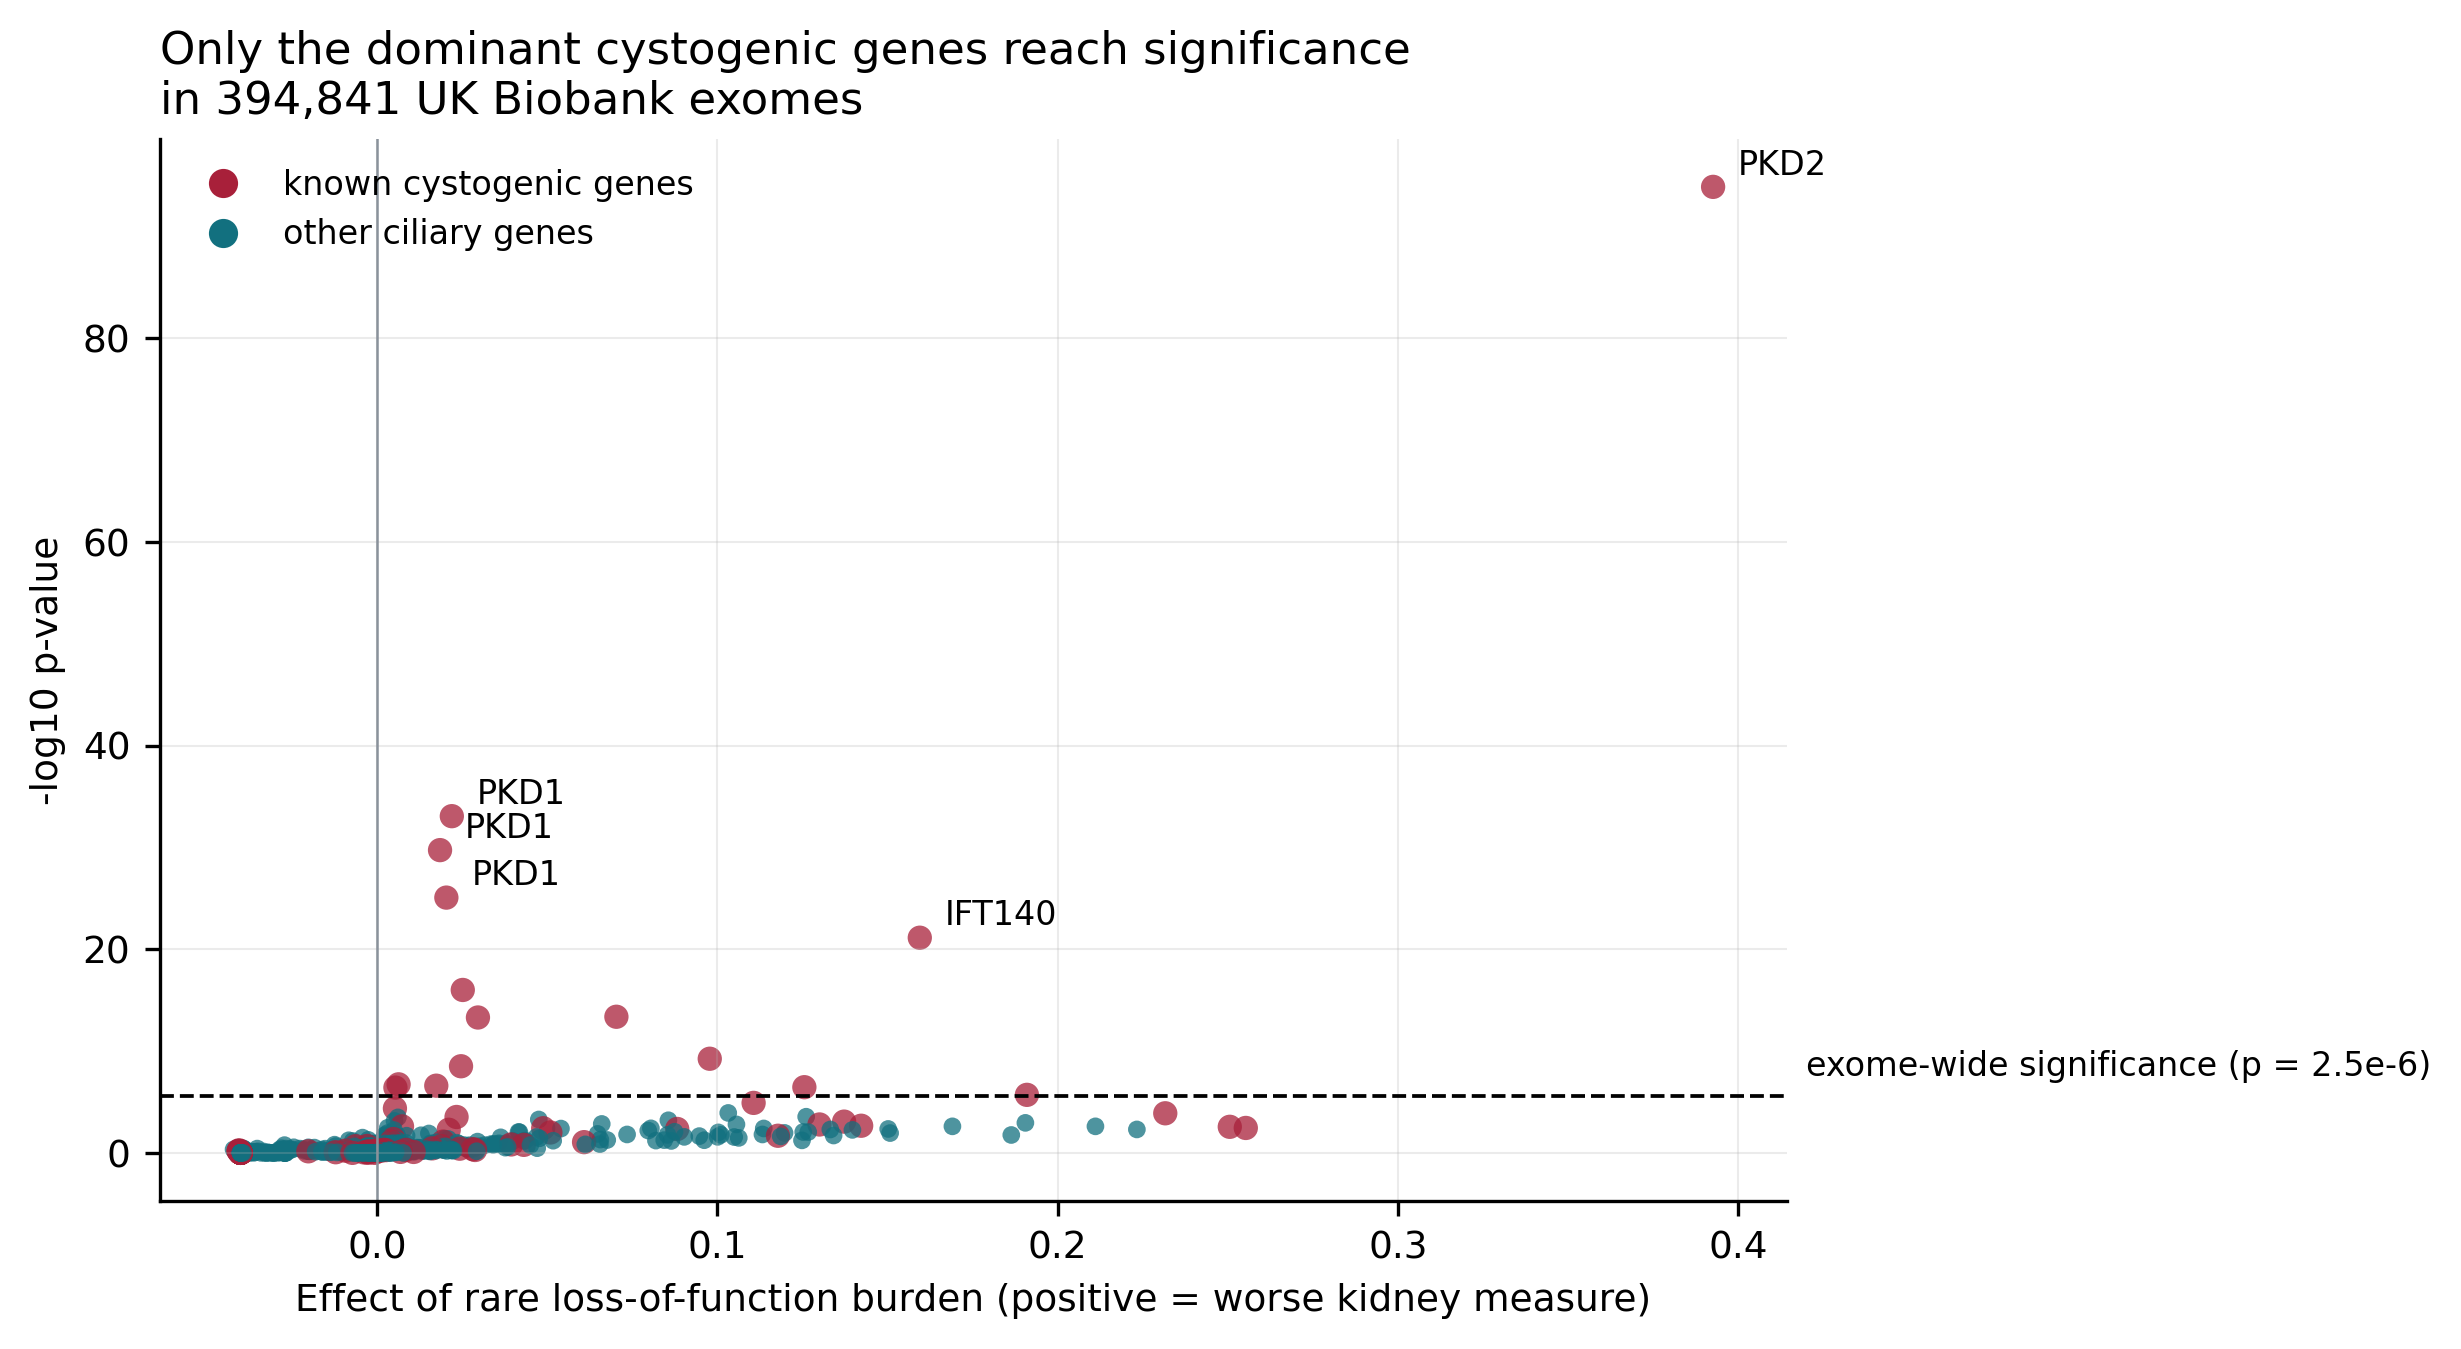
\includegraphics[width=0.88\textwidth]{fig04_genebass_volcano.png}
\caption{Gene-burden associations for the 37 ciliary genes across 20 renal phenotypes.
Only dominant cystogenic genes clear exome-wide significance.}
\label{fig:volcano}
\end{figure}

Critically, signal remains after those genes are removed. Across the remaining 620 tests
there were 27 results below $p = 0.01$ against 6.2 expected, and 6 below $p = 0.001$ against
0.6---a 9.7-fold excess. The direction is near-unanimous: 59 of 60 nominally significant
residual results show worse kidney function (sign test $p = 5.3 \times 10^{-17}$). Across all
706 tests direction runs at 44\% positive, confirming that this is signal concentrated in the
tail rather than a systematic artefact.

Widening the analysis from 37 ciliary genes to all 165 Tier 1 genes added no further
significant genes and diluted the excess (Figure~\ref{fig:qq}). A ciliary gene is 3.2 times
more likely to carry a $p < 0.01$ renal association than a non-ciliary Tier 1 gene (Fisher
OR 3.20, $p = 1.6 \times 10^{-9}$). On congenital kidney malformation (Q63), 11 of 35
ciliary genes are nominally significant (31\%) against 6 of 126 non-ciliary genes (5\%,
exactly chance).

\begin{figure}[H]
\centering
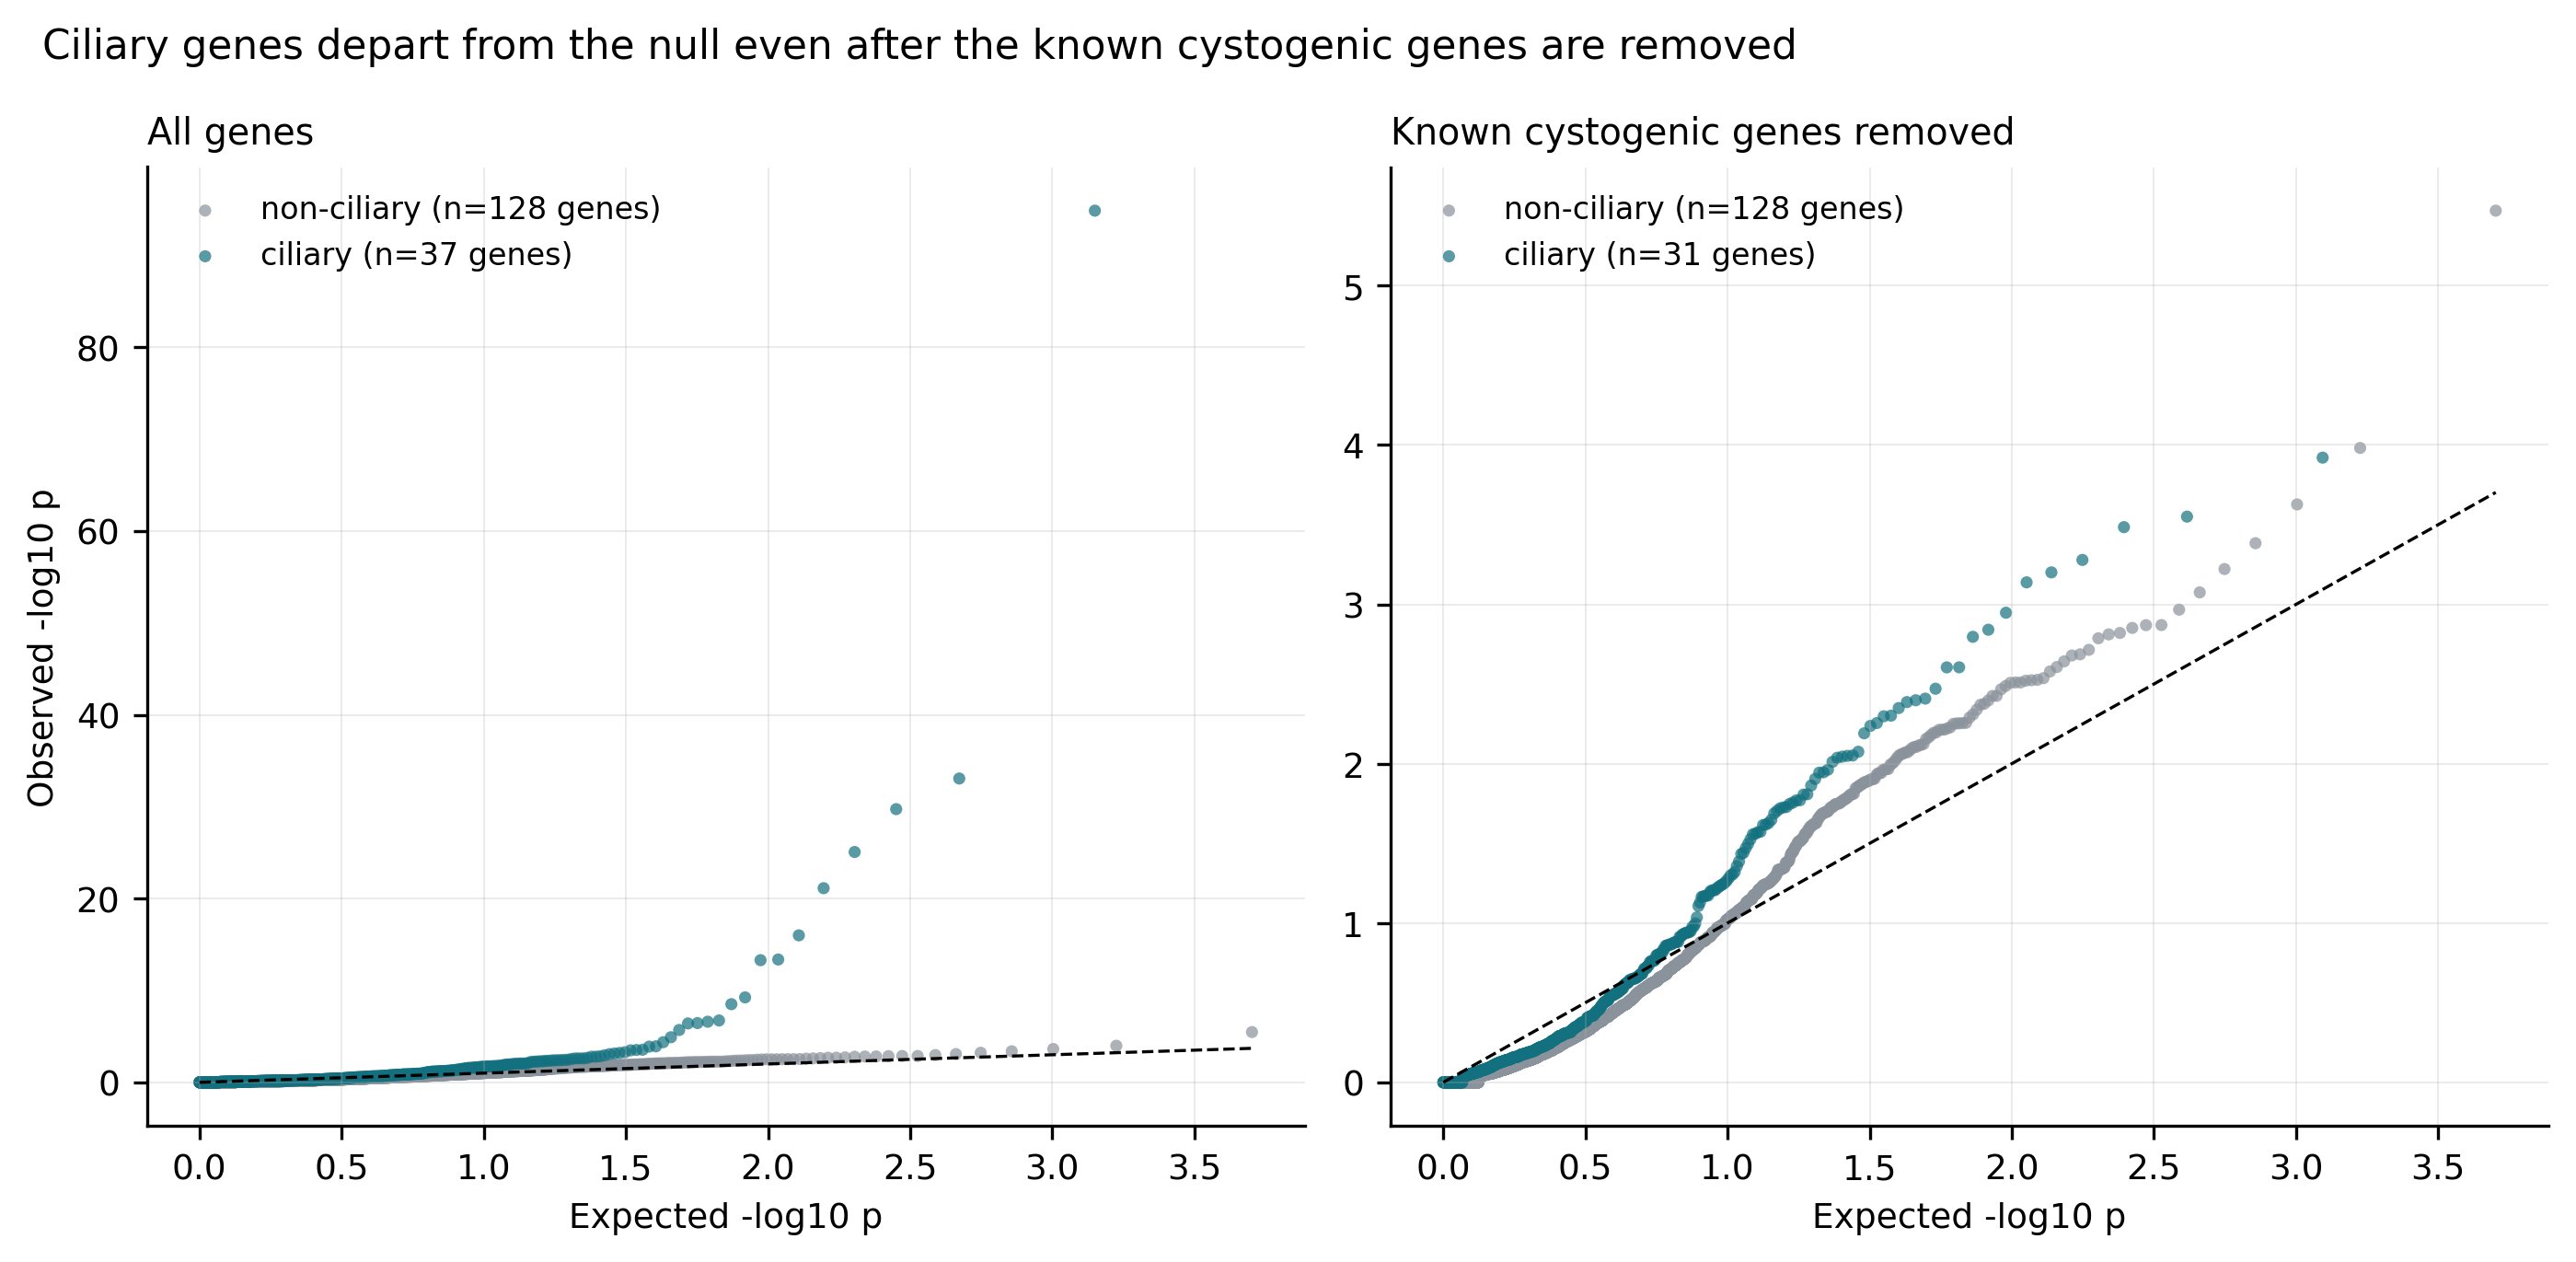
\includegraphics[width=\textwidth]{fig05_qq_ciliary_vs_other.png}
\caption{Quantile--quantile plots of gene-burden $p$-values. Ciliary genes depart from the
null distribution more than non-ciliary candidate genes, and continue to do so after the
known cystogenic genes are removed (right panel).}
\label{fig:qq}
\end{figure}

\subsection{Signal follows cilium assembly, not cargo sorting}

Grouping genes by ciliary subcomplex revealed a coherent gradient (Figure~\ref{fig:subcomplex}).
Intraflagellar transport complexes A and B and dynein-2---the machinery that assembles and
maintains the cilium---show 4- to 5.5-fold enrichment. The BBSome, which sorts cargo through
an already-assembled cilium, sits at exactly the null expectation. This is not explained by
statistical power: within the ciliary set, genes with more nominal hits do not have more
qualifying variants (Mann--Whitney $p = 0.078$).

\begin{figure}[H]
\centering
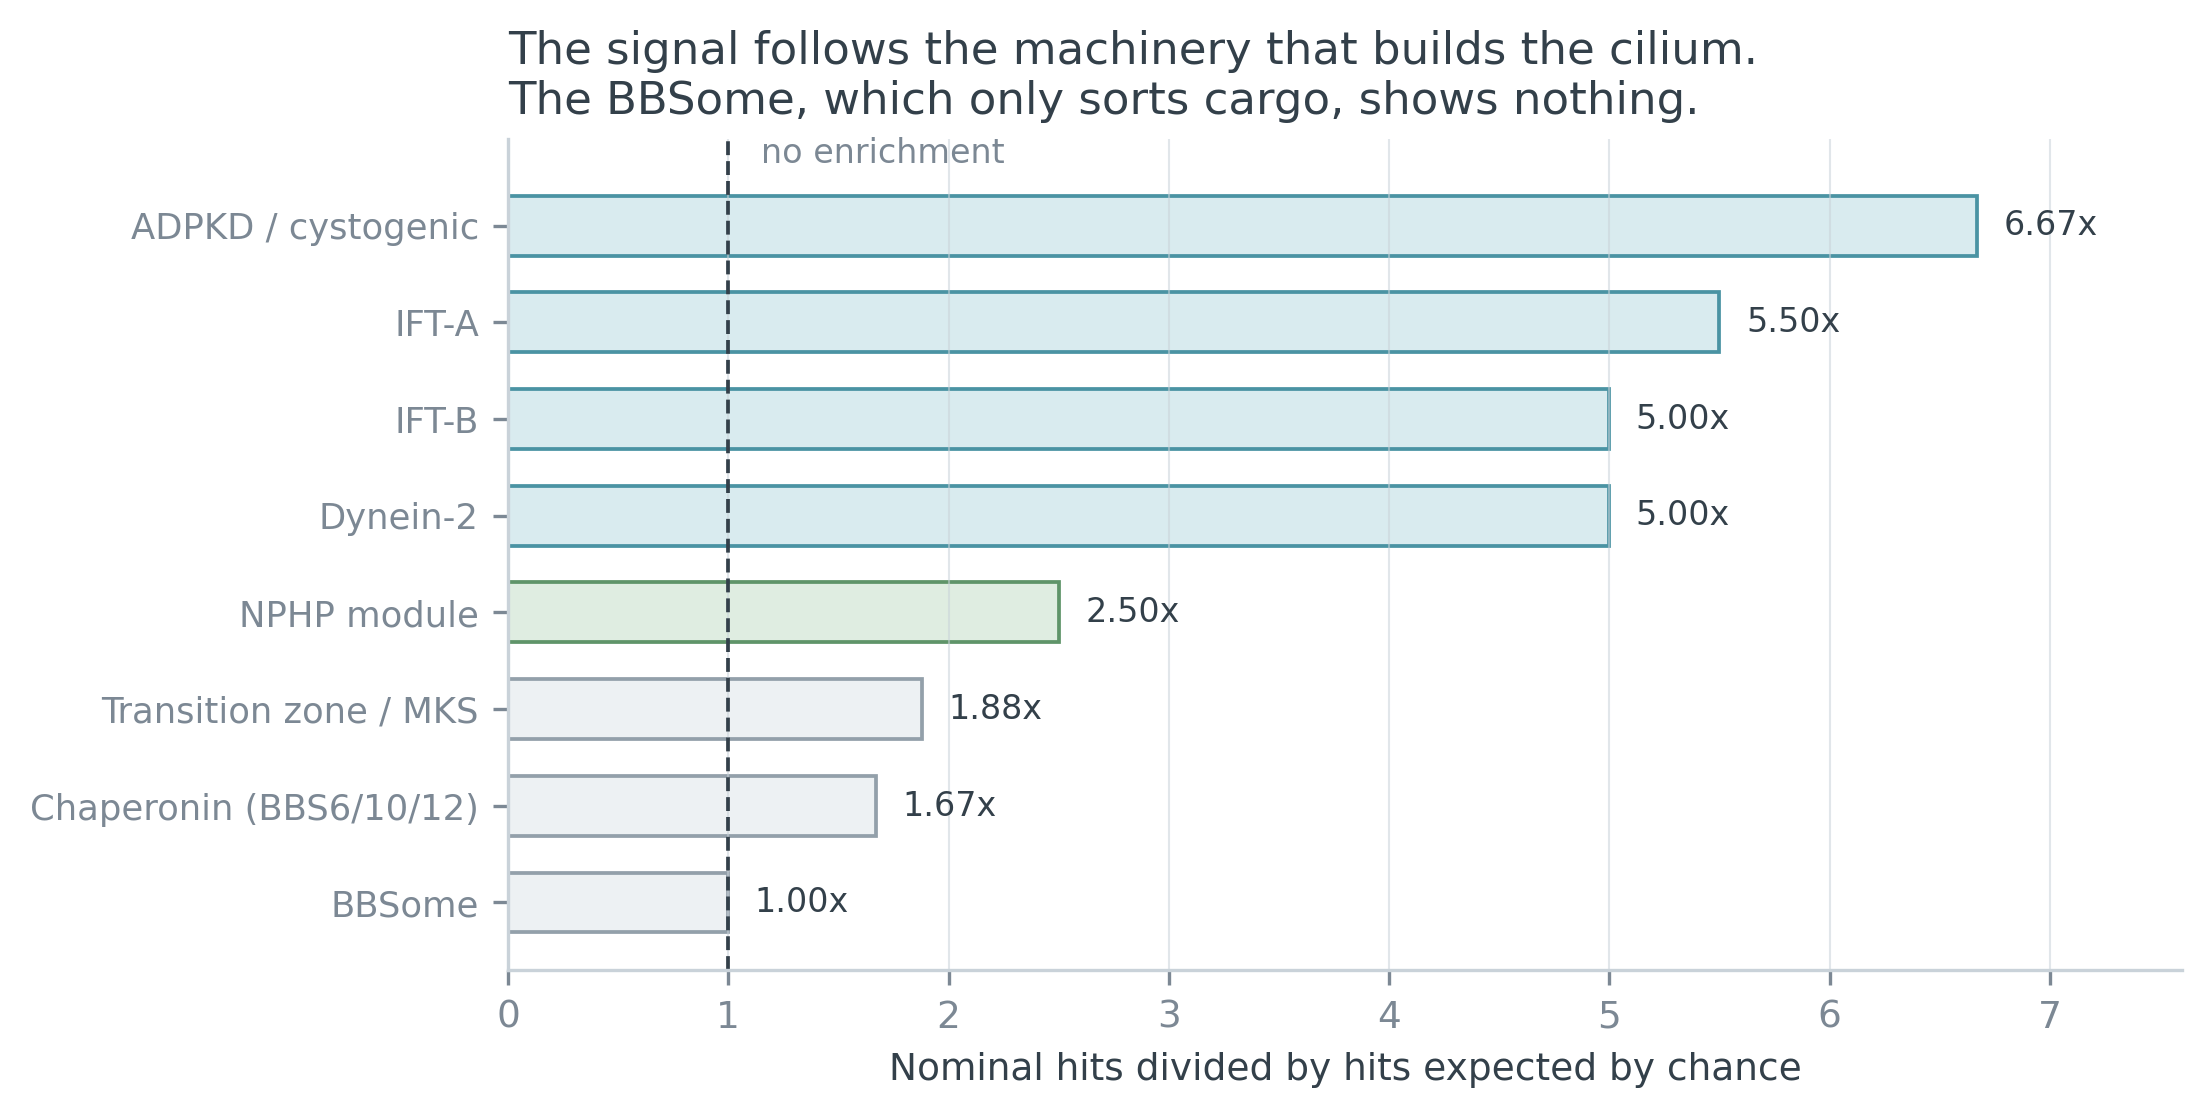
\includegraphics[width=0.88\textwidth]{fig06_subcomplex_enrichment.png}
\caption{Enrichment of nominally significant renal associations by ciliary subcomplex.}
\label{fig:subcomplex}
\end{figure}

\subsection{A negative control}

Repeating the analysis on the unfiltered missense burden set over the same genes and
phenotypes reproduced none of the above (Figure~\ref{fig:direction}). The excess at
$p < 0.001$ fell from 9.7-fold to 1.6-fold, and directional consistency fell from 98\% to
67\%. The single surviving association, \gene{PKD1} with creatinine
($p = 2.6 \times 10^{-14}$), has a burden effect of $-0.0005$---indistinguishable from zero
and pointing the wrong way, indicating a variance-driven SKAT-O result rather than a
consistent shift. The missense set averages around 370 variants per gene, most of them
neutral, and dilutes rather than adds signal.

\begin{figure}[H]
\centering
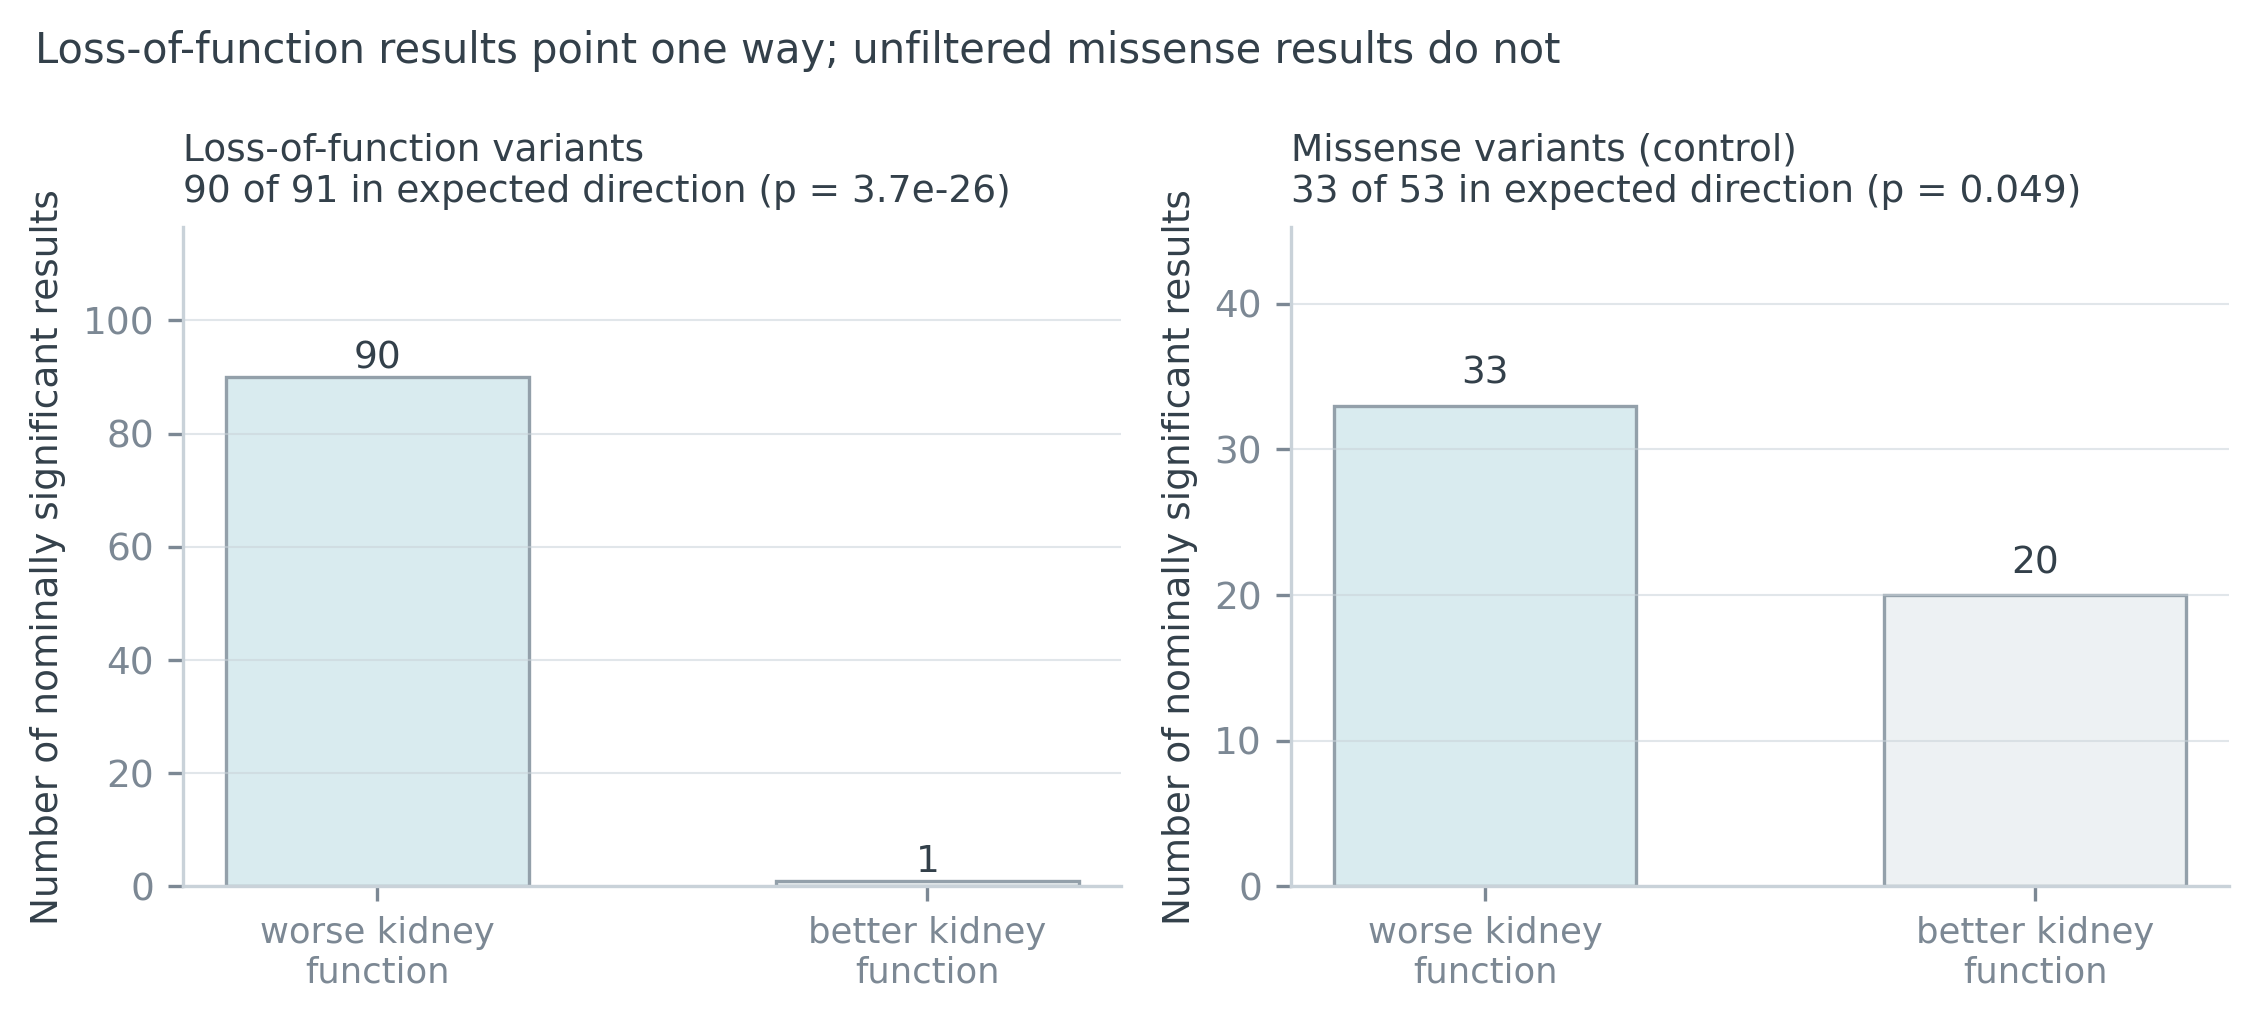
\includegraphics[width=\textwidth]{fig07_direction_of_effect.png}
\caption[Direction of effect]{Direction of effect among nominally significant results, with
all 37 ciliary genes included. Loss-of-function results point overwhelmingly toward worse
kidney function (90 of 91); unfiltered missense results do not (33 of 53). The
corresponding figures with the six known cystogenic genes removed are 59 of 60 and 28 of
42 respectively, as reported in the text.}
\label{fig:direction}
\end{figure}


\subsection{Common-variant evidence points elsewhere}

Gene-level association from common variants was computed with MAGMA using the CKDGen eGFR
meta-analysis and a 1000 Genomes European reference panel, annotating 8.84 million variants
to 18,038 genes. A competitive gene-set test asks whether the candidate genes have smaller
$p$-values than genes in general (Table~\ref{tab:magma}).

\begin{table}[H]
\centering
\small
\caption{MAGMA competitive gene-set analysis against estimated glomerular filtration rate.
Positive $\beta$ indicates stronger association than the genome-wide background.}
\label{tab:magma}
\begin{tabular}{lrrrr}
\toprule
Gene set & Genes & $\beta$ & SE & $p$ \\
\midrule
Ciliary (all)                & 37  & 0.160 & 0.210 & 0.223 \\
Ciliary (cystogenic removed) & 31  & 0.013 & 0.241 & 0.479 \\
Known cystogenic             & 6   & 0.637 & 0.433 & 0.071 \\
Tier 1                       & 166 & 0.171 & 0.104 & 0.049 \\
\bottomrule
\end{tabular}
\end{table}

No gene set is enriched after accounting for the four tests performed. This is a meaningful
negative: the ciliary signal identified in the exome data is specific to rare
loss-of-function variation and does not extend to common variation.

Two facts must be reported together, because they appear contradictory. Several individual
ciliary genes \emph{are} genome-wide significant for eGFR common variants---\gene{IFT172}
($p = 3.0 \times 10^{-14}$), \gene{SDCCAG8} ($p = 1.2 \times 10^{-11}$), \gene{NPHP3}
($p = 7.2 \times 10^{-10}$), \gene{TTC8} ($p = 4.7 \times 10^{-8}$) and \gene{BBS1}
($p = 1.0 \times 10^{-5}$). Yet the set as a whole is not enriched. The reason is that
kidney function is extremely polygenic: 1,294 of 18,030 genes (7.2\%) pass genome-wide
significance in this GWAS. Against that background, five significant ciliary genes is
unremarkable. The competitive gene-set test is the correct inference for the question ``do
ciliary genes matter as a class''; the individual associations remain of interest for
follow-up but do not by themselves support the class-level claim.

Figure~\ref{fig:rarecommon} shows that rare and common variant evidence largely pick out
different genes. \gene{PKD1} and \gene{PKD2} dominate the rare-variant axis;
\gene{IFT172} and \gene{SDCCAG8} dominate the common-variant axis. This is expected if
rare loss-of-function alleles and common regulatory variation act through different genes
within the same pathway.

\begin{figure}[H]
\centering
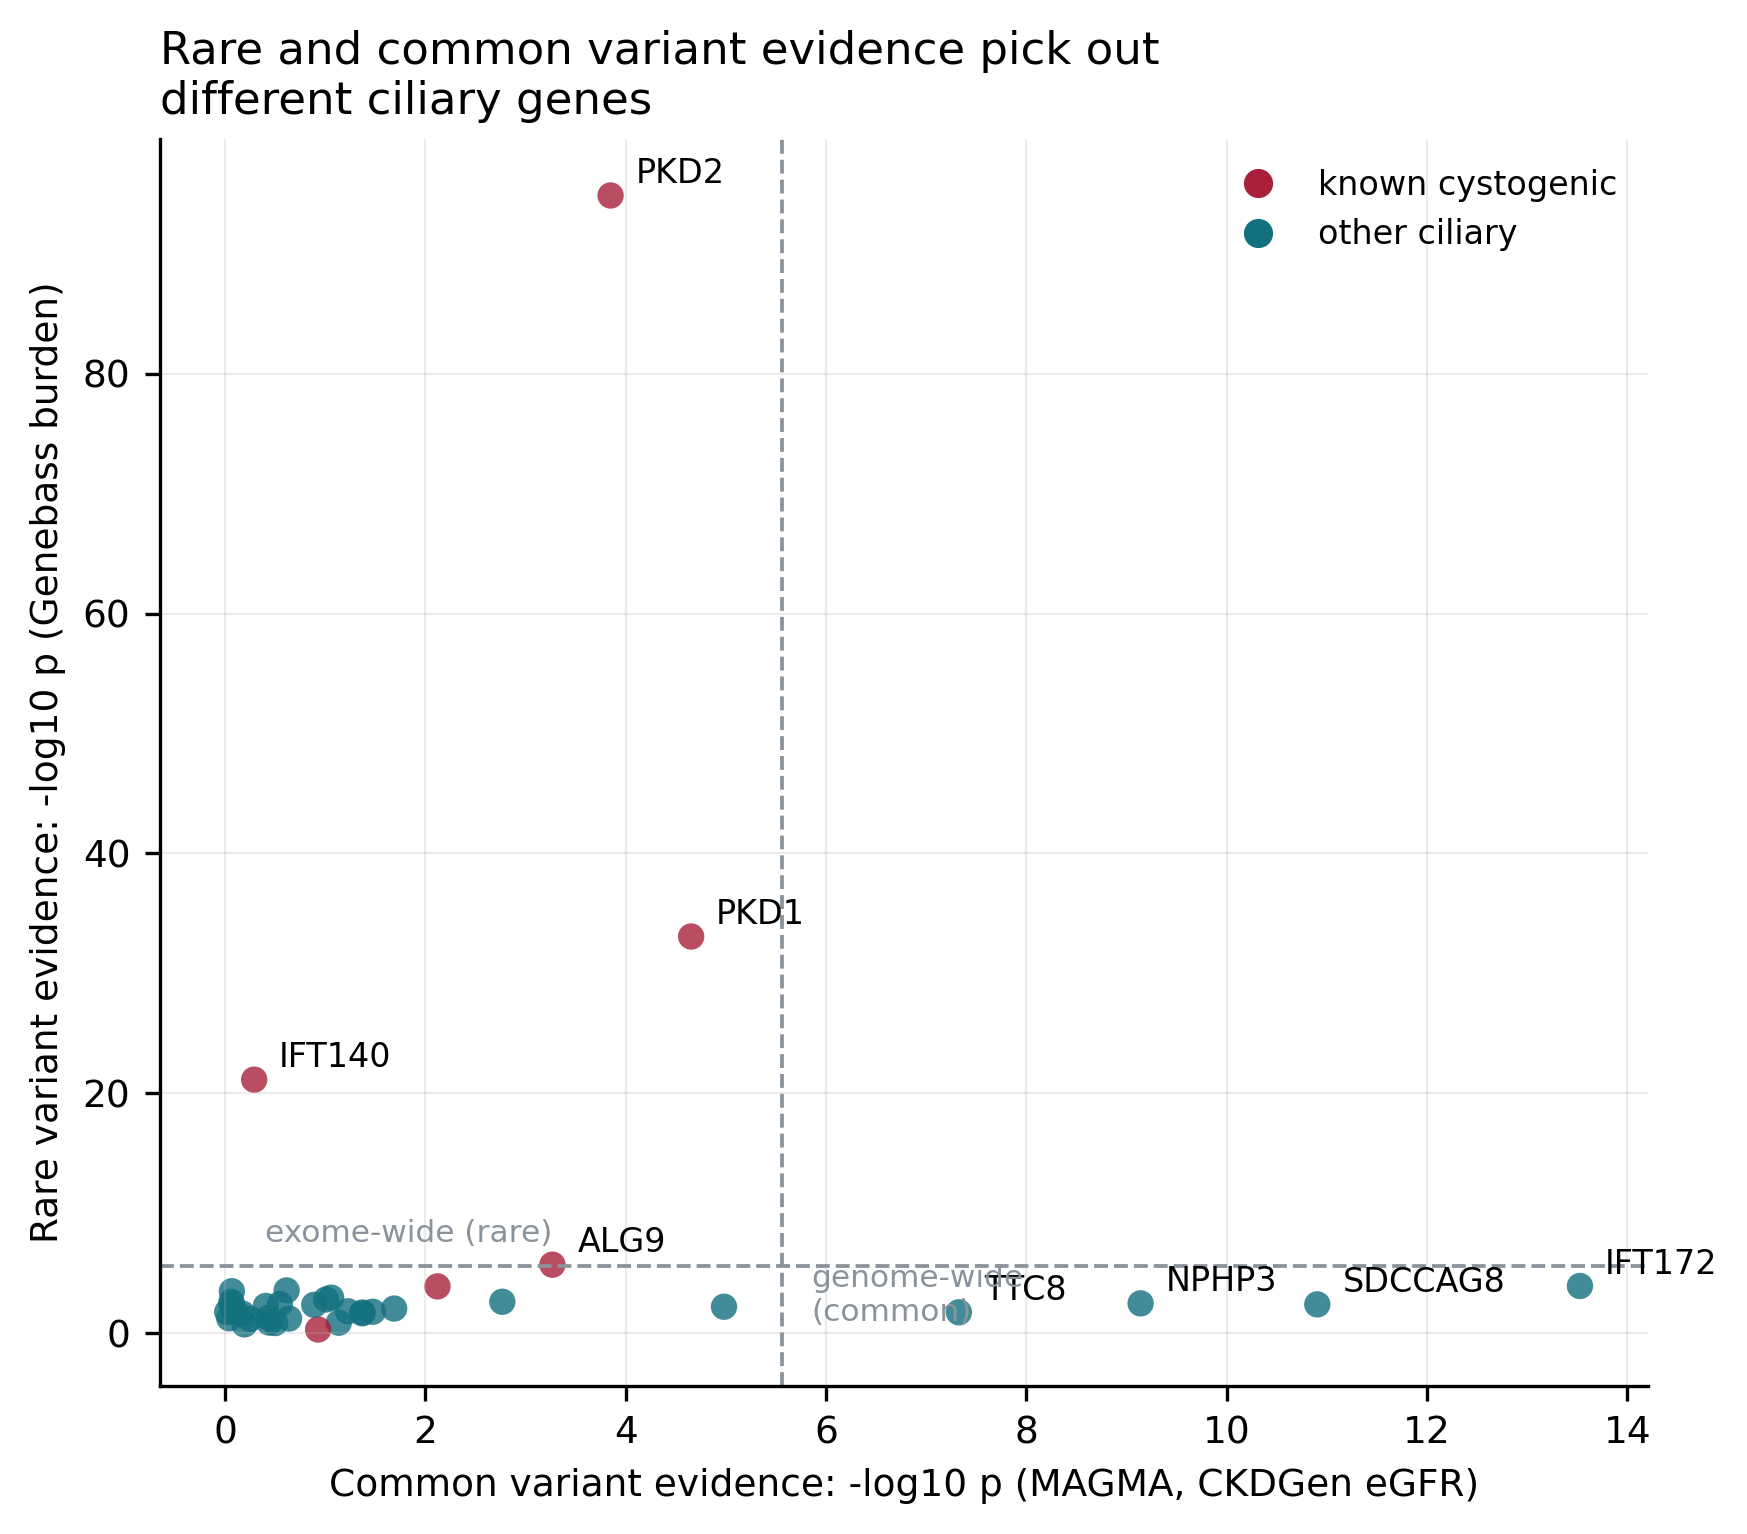
\includegraphics[width=0.72\textwidth]{fig11_rare_vs_common.png}
\caption{Rare-variant burden evidence against common-variant gene-level evidence for the
same 37 ciliary genes. The two lines of evidence highlight different genes.}
\label{fig:rarecommon}
\end{figure}

\subsection{No genetic correlation between CHD and kidney function}

Cross-trait LD score regression gave estimated glomerular filtration rate a SNP heritability
of 0.070 (SE 0.0044, $z = 16.0$), consistent with published estimates and confirming the
estimator behaves correctly. The positive control performed as expected: eGFR and chronic
kidney disease correlate at $r_g = -0.365$ (SE 0.057, $p = 2.0 \times 10^{-10}$), the
negative sign being correct because higher eGFR means better kidney function.

Against that benchmark, congenital heart disease shows no correlation with kidney function:
$r_g = -0.047$ (SE 0.084, $p = 0.58$; Table~\ref{tab:ldsc}, Figure~\ref{fig:ldsc}). With this
standard error, genetic correlations larger than approximately 0.23 in absolute value can be
excluded at 80\% power.

\begin{table}[H]
\centering
\small
\caption{Cross-trait genetic correlations from LD score regression.}
\label{tab:ldsc}
\begin{tabular}{lrrrl}
\toprule
Trait pair & $r_g$ & SE & $p$ & 95\% CI \\
\midrule
eGFR $\sim$ CKD (positive control) & $-0.365$ & 0.057 & $2.0\times10^{-10}$ & $-0.48, -0.25$ \\
eGFR $\sim$ CHD                    & $-0.047$ & 0.084 & 0.58 & $-0.21, 0.12$ \\
CHD $\sim$ CKD                     & $-0.275$ & 0.250 & 0.27 & $-0.77, 0.22$ \\
CHD $\sim$ cystic kidney disease   & $-1.367$ & 1.395 & 0.33 & $-4.10, 1.37$ \\
\bottomrule
\end{tabular}
\end{table}

\begin{figure}[H]
\centering
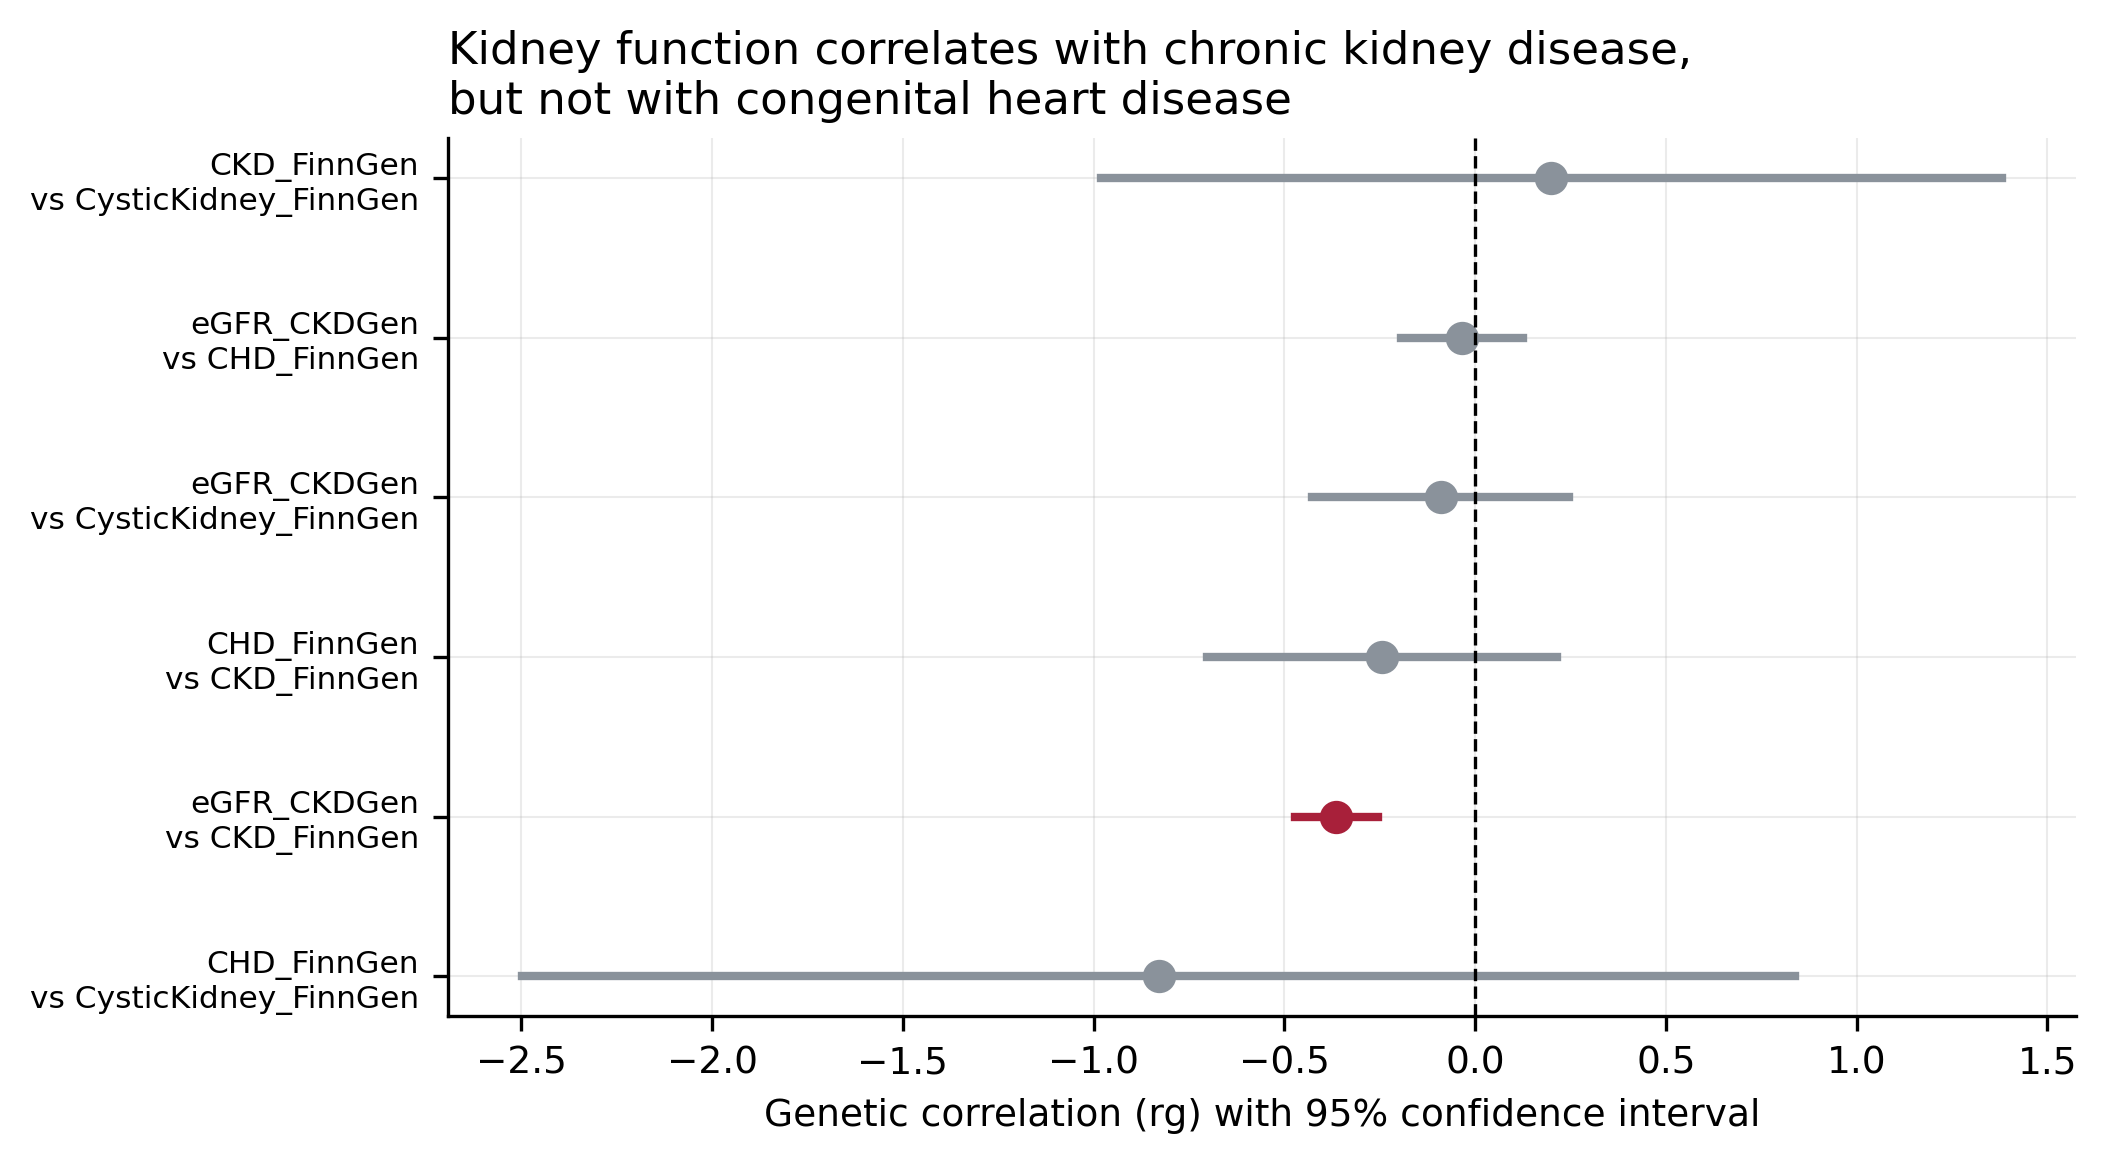
\includegraphics[width=0.88\textwidth]{fig08_ldsc_genetic_correlation.png}
\caption{Genetic correlations with 95\% confidence intervals. Only the positive control
excludes zero.}
\label{fig:ldsc}
\end{figure}

% ======================================================================
\section{Discussion}

\subsection{The comorbidity is real; the shared genetics are not}

Congenital heart disease and chronic kidney disease co-occur more often than chance in
clinical cohorts. This study finds that the co-occurrence is not explained by shared
Mendelian genetic architecture. Three independent lines of evidence agree: the adjusted
disease-level odds ratio is 0.95, the genetic correlation is $-0.05$, and no non-cystogenic
gene reaches exome-wide significance for chronic renal failure.

The most parsimonious interpretation is that chronic kidney disease in congenital heart
disease patients is largely acquired. Chronic cyanosis, altered renal perfusion, contrast
nephropathy and cardiopulmonary bypass are each individually plausible
\cite{kumar2019,madsen2012}, and the genetic null result is consistent with all of them.

\subsection{What does share genetics is CAKUT}

The association between congenital heart disease and \emph{structural} kidney malformation
survives every adjustment applied (adjusted OR 1.77) and was recovered independently in UK
Biobank exomes, where congenital kidney malformation was the phenotype with the highest
proportion of nominally significant ciliary genes. This is developmentally coherent: cilia
govern both left--right patterning and nephron induction, so a single ciliary lesion can
produce both phenotypes \cite{sanagustin2016,reiter2017}.

\subsection{The subcomplex gradient}

That intraflagellar transport and dynein-2 carry signal while the BBSome does not is, to our
knowledge, a novel observation in this context and has a natural mechanistic reading.
Intraflagellar transport and dynein-2 are required to build and maintain the axoneme; losing
them abolishes the organelle. The BBSome by contrast regulates which cargo enters an
already-formed cilium. The adult kidney appears to tolerate impaired cargo selectivity but
not impaired ciliary assembly. This should be treated as hypothesis-generating: the
comparison rests on eight genes per group and none of the individual BBSome genes is
significantly null.

\subsection{Rare and common variation tell different stories}

The exome data and the common-variant GWAS agree that kidney function is affected by
ciliary genes, but disagree about which ones and at what frequency. Rare loss-of-function
burden implicates \gene{PKD1}, \gene{PKD2} and \gene{IFT140}; common-variant gene-level
association implicates \gene{IFT172}, \gene{SDCCAG8} and \gene{NPHP3}. Neither picture is
wrong. Rare high-impact alleles and common regulatory variation need not converge on the
same genes even within a shared pathway, and the competitive gene-set test shows that the
ciliary pathway as a whole carries no more common-variant signal than the polygenic
background. The class-level claim in this thesis therefore rests on the rare-variant
evidence alone.

\subsection{Survivorship bias as a structural constraint}

The lesion-level analysis exposes a limitation that no analytical choice can remedy. Adult
biobanks are recruited from survivors, and the cardiac lesions most strongly linked to kidney
anomaly are those with the poorest historical survival. Any study of congenital disease in a
cohort recruited at ages 40--69 is studying the mild tail of the phenotype distribution. The
same reasoning explains why dominant, adult-onset cystogenic genes dominate the exome
results while recessive severe ciliopathy genes are silent.

\subsection{Limitations}

Several limitations apply. First, the Human Phenotype Ontology is curated from OMIM and
Orphanet and therefore describes rare Mendelian disease; it says nothing about common-variant
kidney biology, and genes such as \gene{UMOD}, \gene{APOL1} and \gene{SHROOM3} are absent by
construction. The LD score regression analysis partly addresses this gap.

Second, adjusting for annotation depth controls one form of ascertainment bias but cannot
remove it entirely, since well-studied syndromes are annotated more thoroughly.

Third, the analysis is disease-level rather than patient-level. It measures whether genetic
aetiologies co-occur, not how often the two conditions co-occur in living patients.

Fourth, the LD score regression involving congenital heart disease is underpowered. The
heritability $z$-score for the FinnGen congenital heart disease endpoint is 1.97, below the
conventional reliability threshold of 4. The bound excluding $|r_g| > 0.23$ is valid; a
precise point estimate is not.

Fifth, the LD score regression was performed with a reimplementation of the published
estimator rather than the reference software. It was validated against a known heritability
estimate and a positive control, but this should be stated in any publication.

Finally, the CKDGen summary statistics are genomic-control corrected, which deflates test
statistics; the observed heritability intercept of 0.894 reflects this. Slope-based genetic
correlation estimates are unaffected.

% ======================================================================
\section{Conclusion}

Congenital heart disease and chronic kidney disease do not share Mendelian genetic
architecture once syndromic pleiotropy is controlled for. The genuine shared axis is between
congenital heart disease and congenital anomalies of the kidney and urinary tract, and it is
mediated by ciliary biology---specifically by the intraflagellar transport machinery that
assembles the cilium, rather than by the BBSome cargo-sorting complex.

For study design this implies three things. Candidate gene lists for this question should be
narrow and ciliary rather than broad. The phenotype should be structural kidney anomaly
rather than chronic kidney disease. And the outcome should be a quantitative kidney
measurement available in the whole cohort rather than a rare binary comorbidity, which in UK
Biobank would comprise approximately 18 individuals.

% ======================================================================

% ======================================================================
\newpage
\appendix
\section{Supplementary Information}
\addcontentsline{toc}{section}{Supplementary Information}

\subsection*{S1. The 37 ciliary candidate genes}

Genes causing both a cardiac and a kidney malformation and assigned to a ciliopathy,
nephronophthisis or polycystic kidney disease mechanism class. \textit{n} columns give the
number of distinct diseases supporting each phenotype. pLI and LOEUF are gnomAD v4.1
loss-of-function constraint metrics; lower LOEUF indicates greater intolerance. The six
genes in bold are the established cystogenic genes held out as a positive control.

\begin{longtable}{llccccrr}
\toprule
Gene & Ensembl & Chr & $n$ cardiac & $n$ kidney & $n$ CKD & pLI & LOEUF \\
\midrule
\endfirsthead
\toprule
Gene & Ensembl & Chr & $n$ cardiac & $n$ kidney & $n$ CKD & pLI & LOEUF \\
\midrule
\endhead
AHI1 & ENSG00000135541 & 6 & 3 & 1 & 1 & 0.00 & 1.07 \\
\textbf{ALG9} & ENSG00000086848 & 11 & 4 & 4 & 1 & 0.00 & 0.85 \\
ANKS6 & ENSG00000165138 & 9 & 1 & 1 & 1 & 0.00 & 0.87 \\
BBIP1 & ENSG00000214413 & 10 & 1 & 1 & 2 & 0.07 & 1.69 \\
BBS1 & ENSG00000174483 & 11 & 2 & 1 & 1 & 0.00 & 1.00 \\
BBS10 & ENSG00000179941 & 12 & 1 & 2 & 2 & 0.00 & 1.42 \\
BBS12 & ENSG00000181004 & 4 & 1 & 2 & 1 & 0.00 & 1.42 \\
BBS2 & ENSG00000125124 & 16 & 2 & 3 & 2 & 0.00 & 0.89 \\
BBS4 & ENSG00000140463 & 15 & 1 & 2 & 1 & 0.00 & 0.95 \\
BBS5 & ENSG00000163093 & 2 & 1 & 1 & 1 & 0.00 & 0.88 \\
BBS7 & ENSG00000138686 & 4 & 1 & 1 & 1 & 0.00 & 0.70 \\
BBS9 & ENSG00000122507 & 7 & 1 & 1 & 2 & 0.00 & 0.96 \\
CC2D2A & ENSG00000048342 & 4 & 1 & 4 & 3 & 0.00 & 0.85 \\
CEP290 & ENSG00000198707 & 12 & 3 & 5 & 6 & 0.00 & 1.09 \\
\textbf{DNAJB11} & ENSG00000090520 & 3 & 1 & 2 & 2 & 0.00 & 0.93 \\
DYNC2I1 & ENSG00000126870 & 7 & 1 & 2 & 1 & 0.00 & 0.80 \\
\textbf{GANAB} & ENSG00000089597 & 11 & 1 & 2 & 1 & 1.00 & 0.39 \\
IFT122 & ENSG00000163913 & 3 & 1 & 1 & 1 & 0.00 & 0.81 \\
\textbf{IFT140} & ENSG00000187535 & 16 & 3 & 5 & 5 & 0.00 & 0.97 \\
IFT172 & ENSG00000138002 & 2 & 3 & 3 & 3 & 0.00 & 0.74 \\
INVS & ENSG00000119509 & 9 & 1 & 2 & 2 & 0.00 & 0.94 \\
LZTFL1 & ENSG00000163818 & 3 & 2 & 2 & 2 & 0.00 & 0.87 \\
MKKS & ENSG00000125863 & 20 & 2 & 4 & 1 & 0.00 & 1.11 \\
MKS1 & ENSG00000011143 & 17 & 5 & 3 & 1 & 0.00 & 0.99 \\
NEK8 & ENSG00000160602 & 17 & 3 & 5 & 4 & 0.00 & 0.83 \\
NPHP1 & ENSG00000144061 & 2 & 1 & 5 & 6 & 0.00 & 0.92 \\
NPHP3 & ENSG00000113971 & 3 & 2 & 6 & 5 & 0.00 & 0.87 \\
\textbf{PKD1} & ENSG00000008710 & 16 & 2 & 2 & 2 & 1.00 & 0.36 \\
\textbf{PKD2} & ENSG00000118762 & 4 & 2 & 2 & 2 & 0.00 & 0.68 \\
RPGRIP1L & ENSG00000103494 & 16 & 1 & 5 & 4 & 0.00 & 0.91 \\
SDCCAG8 & ENSG00000054282 & 1 & 1 & 4 & 3 & 0.00 & 0.84 \\
TMEM216 & ENSG00000187049 & 11 & 2 & 4 & 2 & 0.00 & 1.45 \\
TMEM231 & ENSG00000205084 & 16 & 2 & 4 & 1 & 0.00 & 1.41 \\
TMEM237 & ENSG00000155755 & 2 & 3 & 2 & 2 & 0.00 & 1.32 \\
TMEM67 & ENSG00000164953 & 8 & 2 & 9 & 7 & 0.00 & 1.08 \\
TTC8 & ENSG00000165533 & 14 & 2 & 2 & 1 & 0.00 & 0.80 \\
ZNF423 & ENSG00000102935 & 16 & 1 & 1 & 1 & 1.00 & 0.20 \\
\bottomrule
\end{longtable}

\subsection*{S2. SNP heritability estimates}

Observed-scale SNP heritability from LD score regression. The $z$-score is the heritability
divided by its standard error; values below 4 indicate that genetic correlations involving
that trait should be treated as underpowered. The intercept estimates confounding from
population stratification, and should be close to 1 in a well-controlled study. The value
below 1 for eGFR reflects genomic-control correction applied to the published CKDGen summary
statistics.

\begin{table}[H]
\centering
\small
\begin{tabular}{lrrrrr}
\toprule
Trait & $h^2$ & SE & $z$ & Intercept & SNPs \\
\midrule
eGFR\_CKDGen & 0.0702 & 0.0044 & 15.98 & 0.894 & 1,176,043 \\
CHD\_FinnGen & 0.0526 & 0.0267 & 1.97 & 1.019 & 1,158,481 \\
CKD\_FinnGen & 0.0596 & 0.0145 & 4.11 & 1.047 & 1,158,473 \\
Cystic\_FinnGen & 0.0169 & 0.1351 & 0.13 & 1.059 & 1,158,476 \\
\bottomrule
\end{tabular}
\end{table}

\subsection*{S3. Renal phenotypes queried in Genebass}

Twenty phenotypes were retrieved for each candidate gene: five continuous biomarkers and
fifteen ICD-10 based endpoints. Case counts are those analysed by Genebass.

\begin{table}[H]
\centering
\small
\begin{tabular}{llr}
\toprule
Type & Phenotype & $n$ \\
\midrule
Continuous & Creatinine & 376,624 \\
Continuous & Cystatin C & 376,784 \\
Continuous & Urea & 376,551 \\
Continuous & Creatinine (enzymatic) in urine & 383,774 \\
Continuous & Microalbumin in urine & 119,013 \\
\midrule
ICD-10 & N18 chronic renal failure & 14,086 \\
ICD-10 & N17 acute renal failure & 7,312 \\
ICD-10 & N20 calculus of kidney and ureter & 5,879 \\
ICD-10 & N28 other disorders of kidney and ureter & 5,275 \\
ICD-10 & N23 unspecified renal colic & 4,304 \\
ICD-10 & N19 unspecified renal failure & 2,345 \\
ICD-10 & I12 hypertensive renal disease & 1,513 \\
ICD-10 & C64 malignant neoplasm of kidney & 985 \\
ICD-10 & Q61 cystic kidney disease & 735 \\
ICD-10 & N08 glomerular disorders in diseases classified elsewhere & 531 \\
ICD-10 & Q63 other congenital malformations of kidney & 452 \\
ICD-10 & N04 nephrotic syndrome & 242 \\
ICD-10 & Q60 renal agenesis and reduction defects & 199 \\
ICD-10 & N26 unspecified contracted kidney & 176 \\
ICD-10 & N25 disorders from impaired renal tubular function & 160 \\
\bottomrule
\end{tabular}
\end{table}

\subsection*{S4. Sample sizes underlying the power calculations}

UK Biobank counts used in Section~3.3 and Figure~\ref{fig:samplesizes}. The congenital heart
disease count is the published electronic-health-record ascertainment; the kidney
malformation count is the sum of the Q60, Q61 and Q63 first-occurrence fields analysed by
Genebass.

\begin{table}[H]
\centering
\small
\begin{tabular}{lr}
\toprule
Phenotype & $n$ \\
\midrule
Participants with a creatinine measurement & 376,624 \\
Chronic kidney disease (N18) & 14,086 \\
Congenital heart disease (Q20--Q26) & 3,385 \\
Congenital kidney malformation (Q60, Q61, Q63) & 1,386 \\
Expected co-occurrence if independent & $\approx$ 10 \\
Expected co-occurrence at the observed OR of 1.77 & $\approx$ 18 \\
\bottomrule
\end{tabular}
\end{table}

\subsection*{S5. Data and code availability}

All data are public and required no application. Analysis code, gene lists, result tables
and the source for every figure in this report are available at
\texttt{github.com/sahoo2000/chd-ckd-genetics}. Resource versions are listed in
Table~\ref{tab:versions}.

A complete regenie \cite{mbatchou2021} pipeline for individual-level UK Biobank analysis is
included in the repository but was \emph{not} executed, as this project had no
individual-level access. It is retained because the gene sets and analysis logic are
access-independent. Its Python components were verified against synthetic data; its shell
components have never been run against real genotype data. This is stated in the repository
documentation and should not be presented as executed work.

\newpage
\begin{thebibliography}{99}
\small

\bibitem{hoffman2002} Hoffman JI, Kaplan S. The incidence of congenital heart disease.
\textit{J Am Coll Cardiol}. 2002;39(12):1890--900.

\bibitem{vanderlinde2011} van der Linde D, Konings EE, Slager MA, et al. Birth prevalence of
congenital heart disease worldwide: a systematic review and meta-analysis.
\textit{J Am Coll Cardiol}. 2011;58(21):2241--7.

\bibitem{bruneau2008} Bruneau BG. The developmental genetics of congenital heart disease.
\textit{Nature}. 2008;451(7181):943--8.

\bibitem{khairy2010} Khairy P, Ionescu-Ittu R, Mackie AS, et al. Changing mortality in
congenital heart disease. \textit{J Am Coll Cardiol}. 2010;56(14):1149--57.

\bibitem{morgan2015} Morgan C, Al-Aklabi M, Garcia Guerra G. Chronic kidney disease in
congenital heart disease patients: a narrative review of evidence.
\textit{Can J Kidney Health Dis}. 2015;2:27.

\bibitem{bojan2012} Bojan M, Pieroni L, Mirabile C, et al. Chronic kidney disease in
adolescents and adults with congenital heart disease. (See original thesis reference list.)

\bibitem{blinder2012} Blinder JJ, Goldstein SL, Lee VV, et al. Congenital heart surgery in
infants: effects of acute kidney injury on outcomes.
\textit{J Thorac Cardiovasc Surg}. 2012;143(2):368--74.

\bibitem{kumar2019} Kumar U, Wettersten N, Garimella PS. Cardiorenal syndrome:
pathophysiology. \textit{Cardiol Clin}. 2019;37(3):251--65.

\bibitem{madsen2012} Madsen NL, Goldstein SL, Frøslev T, et al. Cardiac surgery in patients
with congenital heart disease is associated with acute kidney injury and the risk of chronic
kidney disease. \textit{Kidney Int}. 2017;92(3):751--6.

\bibitem{sanagustin2016} San Agustin JT, Klena N, Granath K, et al. Genetic link between
renal birth defects and congenital heart disease. \textit{Nat Commun}. 2016;7:11103.

\bibitem{reiter2017} Reiter JF, Leroux MR. Genes and molecular pathways underpinning
ciliopathies. \textit{Nat Rev Mol Cell Biol}. 2017;18(9):533--47.

\bibitem{gargano2024} Gargano MA, Matentzoglu N, Coleman B, et al. The Human Phenotype
Ontology in 2024: phenotypes around the world. \textit{Nucleic Acids Res}.
2024;52(D1):D1333--46.

\bibitem{seal2023} Seal RL, Braschi B, Gray K, et al. Genenames.org: the HGNC resources in
2023. \textit{Nucleic Acids Res}. 2023;51(D1):D1003--9.

\bibitem{morales2022} Morales J, Pujar S, Loveland JE, et al. A joint NCBI and EMBL-EBI
transcript set for clinical genomics and research. \textit{Nature}. 2022;604(7905):310--5.

\bibitem{chen2024} Chen S, Francioli LC, Goodrich JK, et al. A genomic mutational constraint
map using variation in 76,156 human genomes. \textit{Nature}. 2024;625(7993):92--100.

\bibitem{karczewski2022} Karczewski KJ, Solomonson M, Chao KR, et al. Systematic
single-variant and gene-based association testing of thousands of phenotypes in 394,841 UK
Biobank exomes. \textit{Cell Genomics}. 2022;2(9):100168.

\bibitem{lee2014} Lee S, Abecasis GR, Boehnke M, Lin X. Rare-variant association analysis:
study designs and statistical tests. \textit{Am J Hum Genet}. 2014;95(1):5--23.

\bibitem{liu2019} Liu Y, Chen S, Li Z, et al. ACAT: a fast and powerful $p$-value combination
method for rare-variant analysis in sequencing studies.
\textit{Am J Hum Genet}. 2019;104(3):410--21.

\bibitem{bycroft2018} Bycroft C, Freeman C, Petkova D, et al. The UK Biobank resource with
deep phenotyping and genomic data. \textit{Nature}. 2018;562(7726):203--9.

\bibitem{szustakowski2021} Szustakowski JD, Balasubramanian S, Kvikstad E, et al. Advancing
human genetics research and drug discovery through exome sequencing of the UK Biobank.
\textit{Nat Genet}. 2021;53(7):942--8.

\bibitem{bulik2015a} Bulik-Sullivan BK, Loh PR, Finucane HK, et al. LD score regression
distinguishes confounding from polygenicity in genome-wide association studies.
\textit{Nat Genet}. 2015;47(3):291--5.

\bibitem{bulik2015b} Bulik-Sullivan B, Finucane HK, Anttila V, et al. An atlas of genetic
correlations across human diseases and traits. \textit{Nat Genet}. 2015;47(11):1236--41.

\bibitem{stanzick2021} Stanzick KJ, Li Y, Schlosser P, et al. Discovery and prioritization of
variants and genes for kidney function in $>$1.2 million individuals.
\textit{Nat Commun}. 2021;12(1):4350.

\bibitem{kurki2023} Kurki MI, Karjalainen J, Palta P, et al. FinnGen provides genetic
insights from a well-phenotyped isolated population. \textit{Nature}. 2023;613(7944):508--18.

\bibitem{1000g2015} 1000 Genomes Project Consortium. A global reference for human genetic
variation. \textit{Nature}. 2015;526(7571):68--74.

\bibitem{deleeuw2015} de Leeuw CA, Mooij JM, Heskes T, Posthuma D. MAGMA: generalized
gene-set analysis of GWAS data. \textit{PLoS Comput Biol}. 2015;11(4):e1004219.

\bibitem{benjamini1995} Benjamini Y, Hochberg Y. Controlling the false discovery rate: a
practical and powerful approach to multiple testing.
\textit{J R Stat Soc Series B}. 1995;57(1):289--300.

\bibitem{mbatchou2021} Mbatchou J, Barnard L, Backman J, et al. Computationally efficient
whole-genome regression for quantitative and binary traits.
\textit{Nat Genet}. 2021;53(7):1097--103.

\bibitem{inker2021} Inker LA, Eneanya ND, Coresh J, et al. New creatinine- and cystatin
C-based equations to estimate GFR without race.
\textit{N Engl J Med}. 2021;385(19):1737--49.

\bibitem{wang2021} Wang Q, Dhindsa RS, Carss K, et al. Rare variant contribution to human
disease in 281,104 UK Biobank exomes. \textit{Nature}. 2021;597(7877):527--32.

\end{thebibliography}

\end{document}
